\documentclass[authoryear,preprint,12pt]{elsarticle}

\usepackage{amsmath,amssymb,amsfonts}
\usepackage{lmodern}
\usepackage{graphicx}
\usepackage{booktabs}
\usepackage{tabularx}
\usepackage{multirow}
\usepackage{lineno}
\usepackage{hyperref}
\usepackage{microtype}
\usepackage{adjustbox}
\usepackage{xspace}
\usepackage[margin=2.5cm]{geometry}

% Dynamic results macros generated from reproduction pipeline
% Auto-generated results macros from reproduction pipeline
% DO NOT EDIT DIRECTLY. Generated by scripts/reproduce_paper_2_results.py

\newcommand{\TotalWaterRecords}{268\xspace}
\newcommand{\TotalWaterStudies}{17\xspace}
\newcommand{\TotalMetalRecords}{162\xspace}
\newcommand{\TotalMetalStudies}{12\xspace}
\newcommand{\TotalPhyschemRecords}{106\xspace}
\newcommand{\TotalPhyschemStudies}{5\xspace}
\newcommand{\StudyWindowYears}{2010--2024\xspace}
\newcommand{\LeadWhoExceedPct}{85.6\xspace}
\newcommand{\LeadWhoClusterCi}{[71.1--94.3\%]\xspace}
\newcommand{\LeadWhoWilsonCi}{[79.0--90.4\%]\xspace}
\newcommand{\LeadBdExceedPct}{34.9\xspace}
\newcommand{\LeadBdClusterCi}{[11.4--63.8\%]\xspace}
\newcommand{\LeadBdWilsonCi}{[27.7--43.0\%]\xspace}
\newcommand{\ChromiumWhoExceedPct}{60.6\xspace}
\newcommand{\ChromiumWhoClusterCi}{[32.4--82.8\%]\xspace}
\newcommand{\ChromiumBdExceedPct}{60.6\xspace}
\newcommand{\ArsenicWhoExceedPct}{54.9\xspace}
\newcommand{\ArsenicWhoClusterCi}{[18.1--84.9\%]\xspace}
\newcommand{\ArsenicBdExceedPct}{18.0\xspace}
\newcommand{\ArsenicBdClusterCi}{[1.7--43.4\%]\xspace}
\newcommand{\NickelWhoExceedPct}{54.8\xspace}
\newcommand{\NickelWhoClusterCi}{[21.7--79.1\%]\xspace}
\newcommand{\NickelBdExceedPct}{45.2\xspace}
\newcommand{\CadmiumWhoExceedPct}{44.7\xspace}
\newcommand{\CadmiumWhoClusterCi}{[13.1--77.4\%]\xspace}
\newcommand{\CadmiumBdExceedPct}{40.2\xspace}
\newcommand{\CopperWhoExceedPct}{1.0\xspace}
\newcommand{\CopperBdExceedPct}{6.7\xspace}
\newcommand{\ZincWhoExceedPct}{1.3\xspace}
\newcommand{\ZincBdExceedPct}{0.0\xspace}
\newcommand{\LeadWhoNonUrbanPct}{82.6\xspace}
\newcommand{\LeadBdNonUrbanPct}{18.3\xspace}
\newcommand{\ArsenicBdNonUrbanPct}{8.9\xspace}
\newcommand{\ChromiumWhoNonUrbanPct}{53.0\xspace}
\newcommand{\NickelWhoNonUrbanPct}{32.2\xspace}
\newcommand{\LeadBdNineteenNinetySevenExceedPct}{34.9\xspace}
\newcommand{\LeadBdTwentyTwentyThreeExceedPct}{85.6\xspace}
\newcommand{\CadmiumBdNineteenNinetySevenExceedPct}{40.2\xspace}
\newcommand{\CadmiumBdTwentyTwentyThreeExceedPct}{44.7\xspace}
\newcommand{\NickelBdNineteenNinetySevenExceedPct}{45.2\xspace}
\newcommand{\NickelBdTwentyTwentyThreeExceedPct}{61.5\xspace}
\newcommand{\ArsenicBdNineteenNinetySevenExceedPct}{18.0\xspace}
\newcommand{\ArsenicBdTwentyTwentyThreeExceedPct}{18.0\xspace}
\newcommand{\ChromiumBdNineteenNinetySevenExceedPct}{60.6\xspace}
\newcommand{\ChromiumBdTwentyTwentyThreeExceedPct}{60.6\xspace}
\newcommand{\CopperBdNineteenNinetySevenExceedPct}{6.7\xspace}
\newcommand{\CopperBdTwentyTwentyThreeExceedPct}{1.9\xspace}
\newcommand{\ZincBdNineteenNinetySevenExceedPct}{0.0\xspace}
\newcommand{\ZincBdTwentyTwentyThreeExceedPct}{0.0\xspace}
\newcommand{\LeadConfirmedDissolvedWhoPct}{84.0\xspace}
\newcommand{\ArsenicConfirmedDissolvedWhoPct}{52.4\xspace}
\newcommand{\ChromiumConfirmedDissolvedWhoPct}{55.4\xspace}
\newcommand{\CadmiumConfirmedDissolvedWhoPct}{37.6\xspace}
\newcommand{\NickelConfirmedDissolvedWhoPct}{47.2\xspace}
\newcommand{\LeadConfirmedDissolvedMedian}{0.0250\xspace}
\newcommand{\ChromiumConfirmedDissolvedMedian}{0.0630\xspace}
\newcommand{\NickelConfirmedDissolvedMedian}{0.0560\xspace}
\newcommand{\ArsenicConfirmedDissolvedMedian}{0.0133\xspace}
\newcommand{\CadmiumConfirmedDissolvedMedian}{0.0016\xspace}
\newcommand{\LeadHighSensN}{77\xspace}
\newcommand{\LeadHighSensK}{5\xspace}
\newcommand{\LeadHighSensExceedPct}{79.2\xspace}
\newcommand{\LeadHighSensMedian}{0.0171\xspace}
\newcommand{\HpiCdWeightSharePct}{60.2\xspace}
\newcommand{\HpiPbWeightSharePct}{18.1\xspace}
\newcommand{\HpiAsWeightSharePct}{18.1\xspace}
\newcommand{\HpiCrWeightSharePct}{3.6\xspace}
\newcommand{\HpiCdPbWeightSharePct}{78.3\xspace}
\newcommand{\HpiCoreFourN}{112\xspace}
\newcommand{\HpiCoreFourMedian}{156.99\xspace}
\newcommand{\HpiCoreFourQOne}{69.55\xspace}
\newcommand{\HpiCoreFourQThree}{350.10\xspace}
\newcommand{\HpiCoreFourIqr}{280.55\xspace}
\newcommand{\HpiCoreFourMean}{395.21\xspace}
\newcommand{\HpiCoreFourMax}{2682.05\xspace}
\newcommand{\HpiCoreFourMin}{24.62\xspace}
\newcommand{\HpiCoreFourShareAboveHundred}{58.9\xspace}
\newcommand{\HpiCoreFourShareAboveTwoHundred}{42.9\xspace}
\newcommand{\HpiCommonSubsetCoreFourMedian}{254.13\xspace}
\newcommand{\HpiCommonSubsetCoreFiveMedian}{253.38\xspace}
\newcommand{\HpiCommonSubsetAllSevenMedian}{253.02\xspace}
\newcommand{\HpiHeiSpearmanRho}{0.976\xspace}
\newcommand{\HeiMedian}{6.70\xspace}
\newcommand{\MeanHqMedian}{1.68\xspace}
\newcommand{\DrySeasonRecords}{73\xspace}
\newcommand{\WetSeasonRecords}{28\xspace}
\newcommand{\ExcludedSeasonRecords}{61\xspace}
\newcommand{\ArsenicDryMedian}{0.0073\xspace}
\newcommand{\ArsenicWetMedian}{0.0042\xspace}
\newcommand{\ArsenicDryWetRatio}{1.74\xspace}
\newcommand{\ArsenicTwoSidedP}{0.0039\xspace}
\newcommand{\ArsenicHolmP}{0.0273\xspace}
\newcommand{\ArsenicPremonsoonMedian}{0.0304\xspace}
\newcommand{\ArsenicPremonsoonMean}{0.0632\xspace}
\newcommand{\ArsenicPremonsoonN}{41\xspace}
\newcommand{\ArsenicOverallMedian}{0.0152\xspace}
\newcommand{\ArsenicOverallN}{122\xspace}
\newcommand{\ArsenicWithinStudyK}{4\xspace}
\newcommand{\ArsenicWithinStudyRatio}{1.43\xspace}
\newcommand{\ArsenicWithinStudyHksjCi}{[0.60--3.41]\xspace}
\newcommand{\LeadWithinStudyRatio}{1.28\xspace}
\newcommand{\LeadWithinStudyHksjCi}{[0.56--2.95]\xspace}
\newcommand{\TotalMajorReachesCount}{2224\xspace}
\newcommand{\TotalMajorLengthKm}{4599.1\xspace}
\newcommand{\UniqueStationCoordinates}{23\xspace}
\newcommand{\ObservedCoveredLengthKm}{757.2\xspace}
\newcommand{\ObservedCoveredPct}{16.5\xspace}
\newcommand{\UnsampledCountTwentyFiveKm}{1890\xspace}
\newcommand{\UnsampledPctCountTwentyFiveKm}{85.0\xspace}
\newcommand{\UnsampledLengthTwentyFiveKm}{3841.9\xspace}
\newcommand{\UnsampledPctLengthTwentyFiveKm}{83.5\xspace}
\newcommand{\UnsampledPctLengthTenKm}{95.2\xspace}
\newcommand{\UnsampledPctLengthFiftyKm}{59.4\xspace}
\newcommand{\UnsampledPctLengthNetworkTwentyFiveKm}{89.0\xspace}
\newcommand{\NullModelMeanCoveragePct}{38.2\xspace}
\newcommand{\NullModelCiLoPct}{32.1\xspace}
\newcommand{\NullModelCiHiPct}{44.5\xspace}
\newcommand{\NullModelPval}{0.0000\xspace}
\newcommand{\NullModelPvalFormatted}{\le 0.001\xspace}


\journal{Environmental Pollution}

\begin{document}

\begin{frontmatter}

\title{Heavy Metals in Monitored River Corridors of Bangladesh: A Critical Synthesis of Published Records (\StudyWindowYears), Regulatory Benchmark Discordance, and Hydrographic Surveillance Deficits}

\author[inst1]{Author One\corref{cor1}}
\ead{author.one@university.edu}
\author[inst1,inst2]{Author Two}
\ead{author.two@institution.org}
\author[inst2]{Author Three}
\ead{author.three@research.org}

\cortext[cor1]{Corresponding author. E-mail: author.one@university.edu}

\affiliation[inst1]{organization={Department of Environmental Science and Engineering},
            addressline={University Name}, 
            city={Dhaka},
            postcode={1000},
            country={Bangladesh}}

\affiliation[inst2]{organization={Institute of Water and Flood Management},
            addressline={Technical University}, 
            city={Dhaka},
            postcode={1205},
            country={Bangladesh}}

\begin{abstract}
Surface freshwater in the Bengal Delta provides indispensable resources for ecology, agriculture, and municipal water abstraction, but fluvial corridors receive substantial untreated industrial and municipal effluents. Here, we present a critical synthesis and benchmark audit of published heavy metal records across monitored Bangladesh river corridors by evaluating \TotalMetalRecords\ trace element records across \TotalMetalStudies\ peer-reviewed investigations published between \StudyWindowYears\ (alongside 106 bulk physicochemical records across 5 investigations cataloged during systematic study reconciliation). We screen raw river water concentrations against international health benchmarks (WHO Guidelines for Drinking-water Quality, 4th ed.\ incorporating 2022 addenda), historical national standards (Bangladesh Environmental Conservation Rules, ECR 1997 Schedule 3), contemporary national standards (ECR 2023 Schedule 2, S.R.O. 53-Law/2023), and agricultural irrigation criteria (FAO Paper 29) to evaluate ambient chemical pressure and water treatment burdens on municipal abstraction facilities. Accounting for study-level clustering via 5,000-resample cluster bootstrapping and random-effects meta-analysis, widespread benchmark exceedances are documented in published literature: Lead (Pb) exceeded the WHO potable guideline (0.010~mg/L) in \textbf{\LeadWhoExceedPct\%} of records (study-level cluster 95\% CI: \LeadWhoClusterCi; median: 0.0286~mg/L; random-effects pooled proportion: 79.9\% [95\% CI: 57.4--92.2\%]). Under the superseded ECR 1997 standard (0.050~mg/L), Pb exceedance was \textbf{\LeadBdNineteenNinetySevenExceedPct\%} (\LeadBdClusterCi), but under the updated ECR 2023 Schedule 2 potable limit (0.010~mg/L), national potable benchmark exceedance rises to \textbf{\LeadBdTwentyTwentyThreeExceedPct\%}, harmonizing with the WHO guideline. Regulatory tightening under ECR 2023 also increased potable exceedance for Cadmium (0.005 to 0.003~mg/L; \CadmiumBdNineteenNinetySevenExceedPct\% to \CadmiumBdTwentyTwentyThreeExceedPct\%) and Nickel (0.100 to 0.050~mg/L; \NickelBdNineteenNinetySevenExceedPct\% to \NickelBdTwentyTwentyThreeExceedPct\%). Evaluating confirmed dissolved records (0.45~$\mu\text{m}$ filtered; $k=10$ studies) demonstrated that elevated concentrations persist in the dissolved phase (median Pb: \LeadConfirmedDissolvedMedian~mg/L; \LeadConfirmedDissolvedWhoPct\% exceedance; Cr: \ChromiumConfirmedDissolvedMedian~mg/L; As: \ArsenicConfirmedDissolvedMedian~mg/L), corroborated under high-sensitivity spectrometry (GF-AAS/ICP-MS: \LeadHighSensExceedPct\% Pb exceedance, median \LeadHighSensMedian~mg/L). Mathematical decomposition of the Heavy Metal Pollution Index ($\mathrm{HPI}$) demonstrates that because sub-indices and weights both scale inversely with standards ($W_i \propto 1/S_i, Q_i \propto 1/S_i$), index scores scale quadratically with $M_i/S_i^2$, concentrating 78.3\% of Core-4 linear weights and 77.1\% of median index scores onto Cd and Pb. This algebraic damping explains observed panel invariance on identical common subsets ($N=35$; Core-4 median: \HpiCommonSubsetCoreFourMedian, Core-5: \HpiCommonSubsetCoreFiveMedian, All-7: \HpiCommonSubsetAllSevenMedian; full $N=112$ Core-4 median: \HpiCoreFourMedian). In seasonal contrasts, paired within-study meta-analyses incorporating Hartung-Knapp-Sidik-Jonkman (HKSJ) adjustments ($k=3\text{--}5$) yielded 95\% confidence intervals spanning unity across all seven metals (Pb ratio \LeadWithinStudyRatio$\times$ [\LeadWithinStudyHksjCi]; As \ArsenicWithinStudyRatio$\times$ [\ArsenicWithinStudyHksjCi]), indicating that within-study seasonal variations cannot be declared statistically significant with small paired study counts, while resolving an apparent Arsenic median paradox via a tripartite hydrological distribution (pre-monsoon summer irrigation pumping peak: median \ArsenicPremonsoonMedian~mg/L, $N=41$; dry winter: \ArsenicDryMedian~mg/L; wet monsoon: \ArsenicWetMedian~mg/L). Finally, topological stream routing across HydroSHEDS HydroRIVERS reaches strictly within Bangladesh (\TotalMajorReachesCount\ reaches totaling \TotalMajorLengthKm~km) demonstrated that compiled academic sites cover only \ObservedCoveredPct\% of major river length (\ObservedCoveredLengthKm~km) at 25~km (\UnsampledPctLengthTwentyFiveKm\% length uncovered; \UnsampledPctLengthNetworkTwentyFiveKm\% along-network), which is significantly lower than spatial random expectation (\NullModelMeanCoveragePct\%, Monte Carlo $p \le 0.001$). These findings establish that published data characterize monitored urban-industrial pressure corridors rather than national baseline waters, and highlight critical surveillance deficits across the delta.
\end{abstract}

\begin{graphicalabstract}
\centering
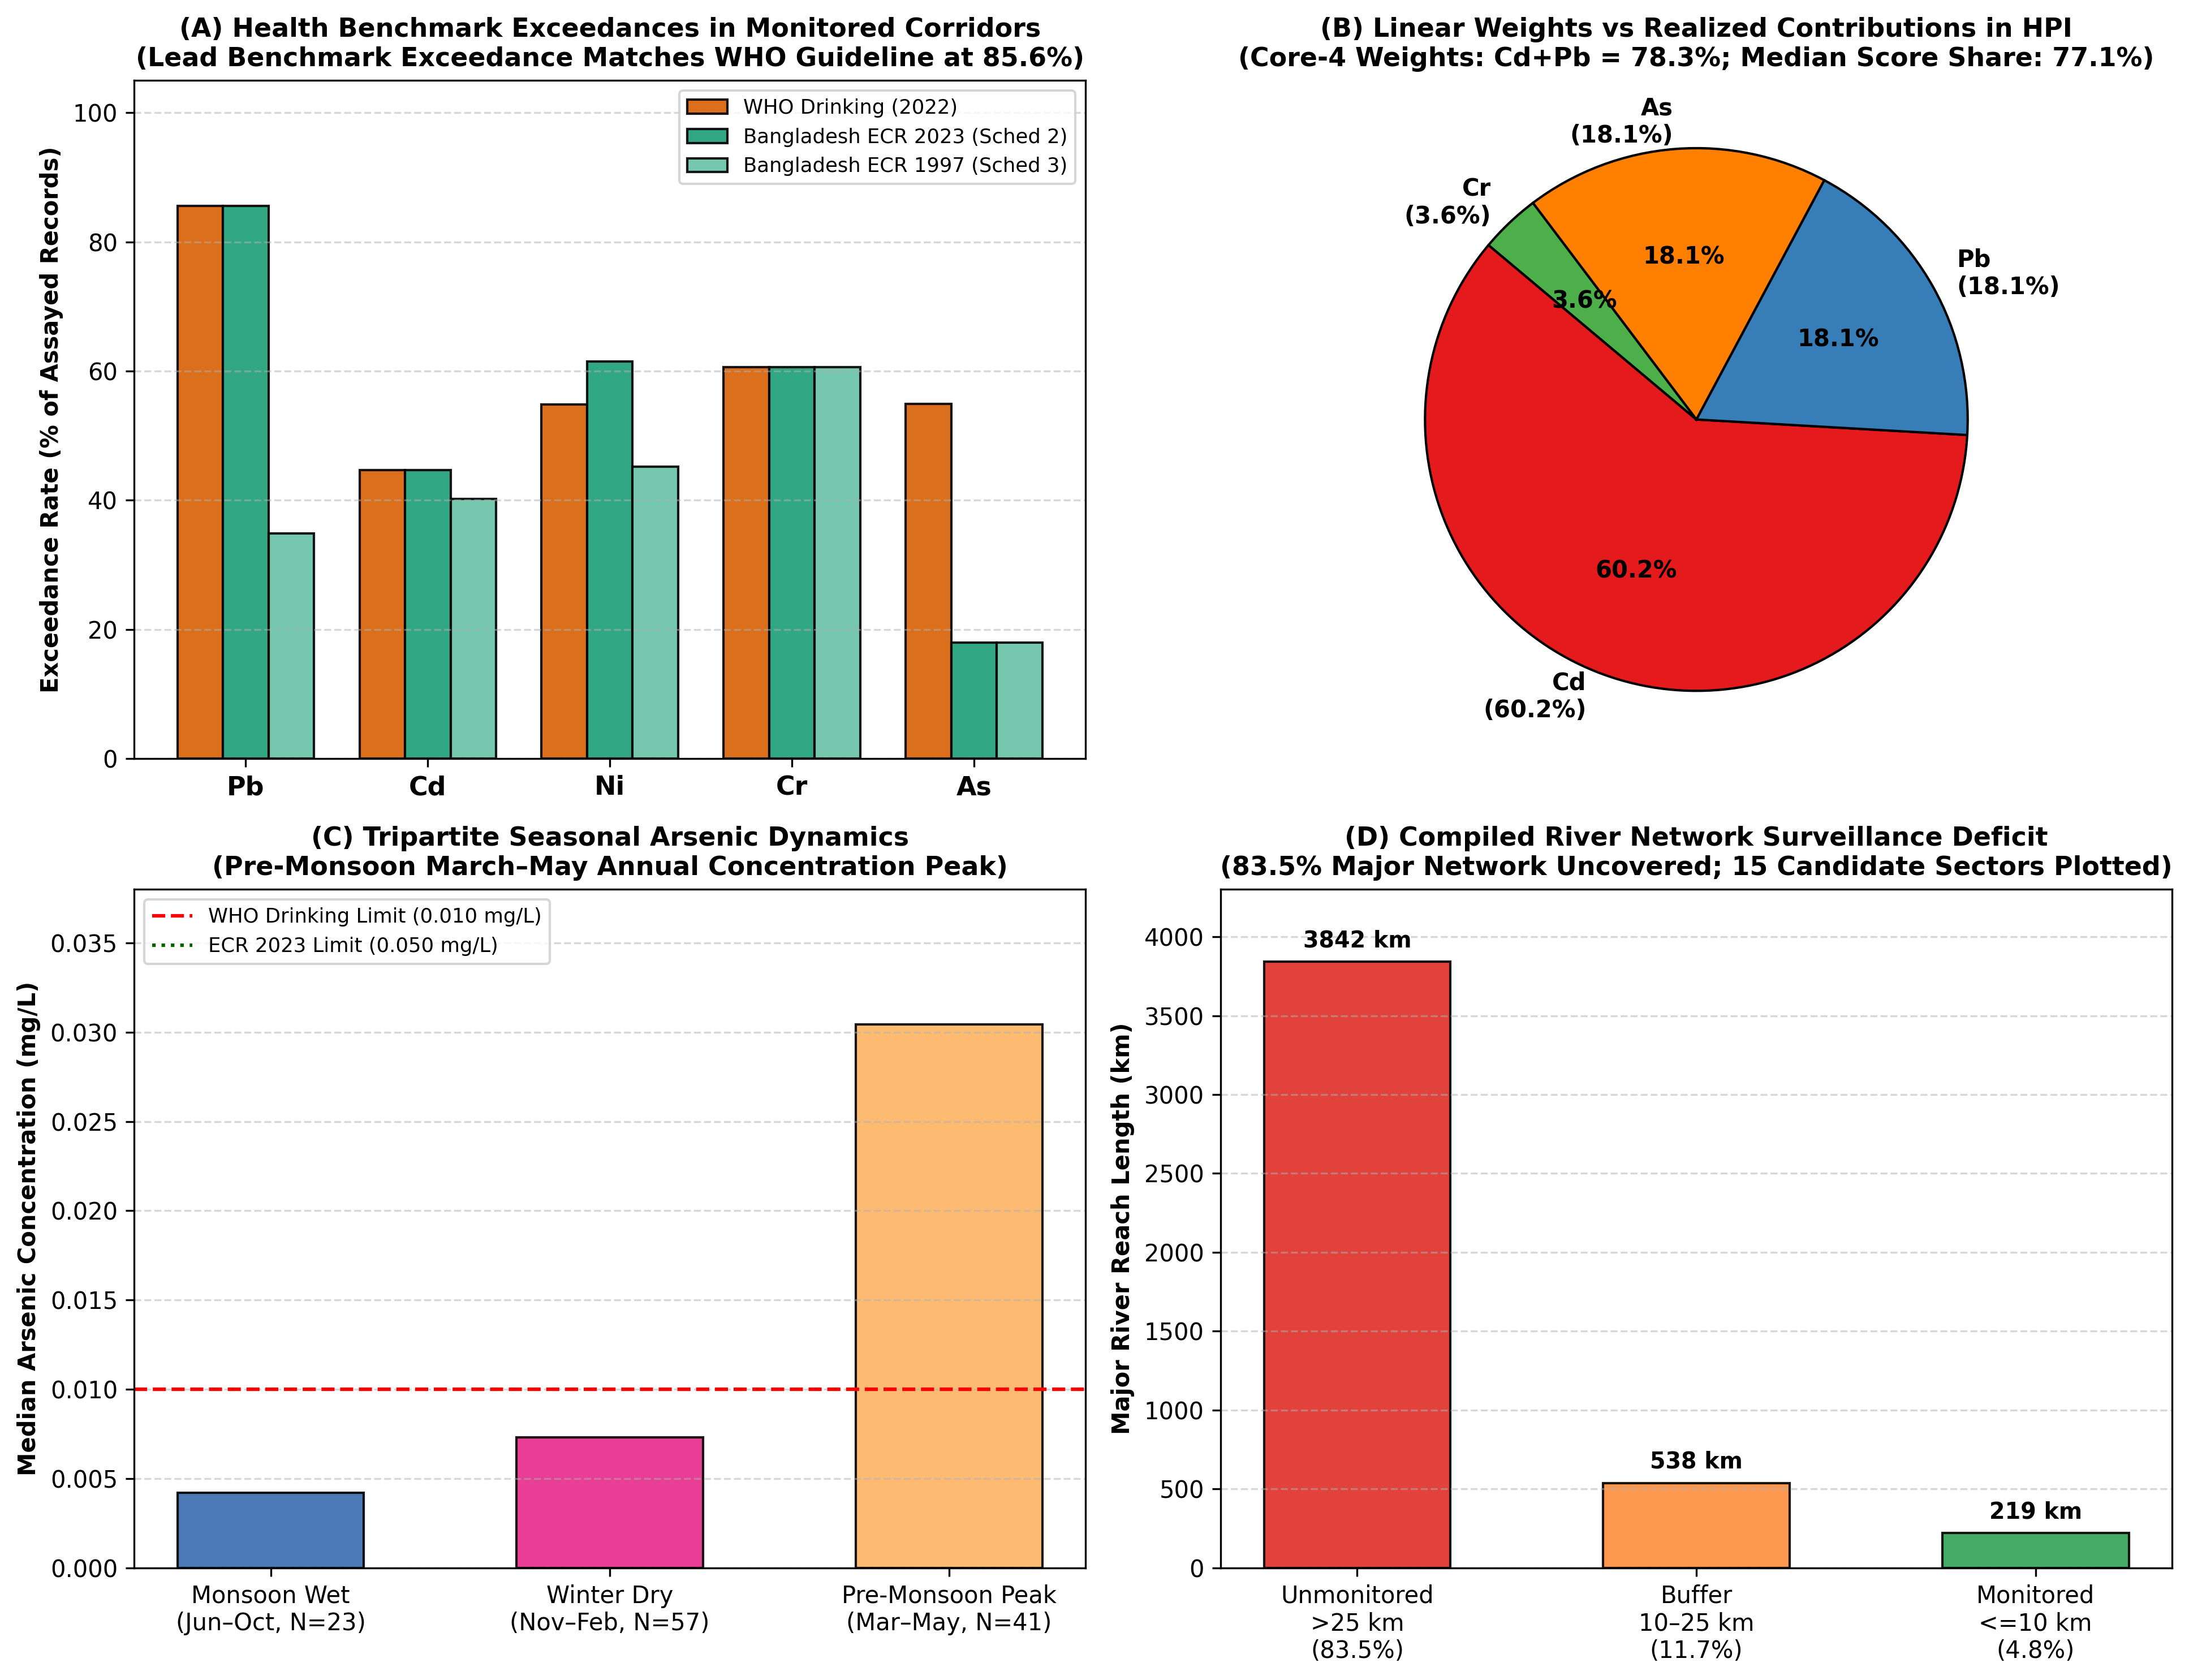
\includegraphics[width=0.98\textwidth]{graphical_abstract.png}
\end{graphicalabstract}

\begin{highlights}
\item Pb exceeds WHO drinking guideline in 85.6\% of compiled records.
\item Updated ECR 2023 drinking limit aligns with WHO, raising Pb exceedance.
\item High-sensitivity spectrometry confirms 79.2\% Pb drinking exceedance.
\item HPI scales with $1/S_i^2$, placing 78\% of linear weight on Cd and Pb.
\item Compiled academic sites cover only 16.5\% of major river length.
\end{highlights}

\begin{keyword}
River water \sep Trace elements \sep Drinking water benchmarks \sep ECR 2023 \sep Heavy Metal Pollution Index ($\mathrm{HPI}$) \sep Seasonal contrast \sep Spatial coverage
\end{keyword}

\end{frontmatter}

\linenumbers

\section{Introduction}
Surface freshwater networks formed by the Ganges, Brahmaputra, and Meghna (GBM) river basins support approximately 169.8 million people in Bangladesh \citep{BBS2022}, sustaining irrigated agriculture, capture fisheries, municipal intake facilities, and industrial supply \citep{Chowdhury2004}. However, rapid industrial growth across the textile dyeing, leather tanning, pharmaceutical, and chemical manufacturing sectors, combined with untreated municipal discharges, has introduced significant toxic contaminants into fluvial corridors \citep{Bhuiyan2015,Islam2015}.

Among aquatic pollutants, heavy metals and metalloids (e.g., As, Cd, Cr, Cu, Ni, Pb, Zn) present persistent environmental health concerns because of their non-biodegradability and potential for trophic transfer \citep{Jarup2003,Tchounwou2012}. Chronic ingestion or exposure to elevated trace element levels can cause nephrotoxicity, neurodevelopmental deficits, and cardiovascular diseases \citep{Needleman2004,Saha2017}. To protect public health and aquatic ecosystems, the World Health Organization \citep{WHO2022}, the Bangladesh Department of Environment \citep{ECR1997,ECR2023}, and the Food and Agriculture Organization \citep{FAO1985} have established concentration benchmarks. While untreated surface river water is ambient freshwater rather than finished tap water delivered at the point of consumption, screening raw river concentrations against potable and irrigation benchmarks provides a transparent screening metric of ambient chemical pressure and treatment burden on municipal surface water abstraction facilities \citep{Islam2015,Li2018}.

Previous review articles have summarized heavy metal occurrences across environmental matrices in Bangladesh \citep{Islam2018review} or reported broad multi-decade water quality indices \citep{Bilal2023,Proshad2025}. However, prior multi-river compilations frequently pooled disparate study observations without accounting for intra-study clustering, did not document non-detect detection-limit censoring, evaluated pollution indices on shifting metal panels that artificially altered index scores, and lacked spatial validation against hydrological reach networks. The present study directly addresses these methodological challenges by providing: (i) an audited, provenance-documented dataset reconciling 28 primary investigations with explicit non-detect handling; (ii) cluster-robust bootstrap confidence intervals and random-effects meta-analytic pooling with prediction intervals; (iii) a standardized Core-4 fixed-panel HPI formulation validated across identical common subsets alongside mathematical decomposition of index scaling; (iv) paired within-study seasonal contrasts evaluated alongside pooled tests with small-sample adjustments; and (v) an empirical spatial coverage evaluation against the HydroSHEDS river network with an explicit Monte Carlo spatial null model.

To address these questions, this study presents an audited descriptive synthesis of published river water records (\StudyWindowYears) across Bangladesh to:
\begin{enumerate}
    \item Screen trace element concentrations against WHO reference guidelines, Bangladesh statutory standards, and FAO irrigation limits, incorporating unadjusted Wilson score intervals, 5,000-resample study-level cluster bootstrap confidence intervals, random-effects meta-analysis proportions with prediction intervals, instrument stratification, and sensitivity analyses excluding urban industrial hotspots.
    \item Evaluate multi-metal water pollution status using the Heavy Metal Pollution Index ($\mathrm{HPI}$) computed on a standardized fixed core panel (As, Cd, Cr, Pb), establishing comparability against the Heavy Metal Evaluation Index ($\mathrm{HEI}$) and evaluating same-subset panel stability and mathematical weighting behavior.
    \item Statistically evaluate dry-versus-wet seasonal contrasts using within-study random-effects meta-analysis of log-ratios alongside pooled non-parametric hypothesis testing with Holm-Bonferroni corrections and tripartite hydrological partitioning.
    \item Quantify the spatial coverage of published sampling sites along major river reaches using straight-line (Haversine) and along-network topological stream distances in HydroSHEDS HydroRIVERS evaluated against a spatial Monte Carlo null model.
\end{enumerate}

\section{Materials and Methods}

\subsection{Literature Compilation, PRISMA Screening, and QA/QC Audit Protocol}
A systematic literature compilation was conducted according to PRISMA principles across peer-reviewed investigations published between 2010 and 2024 reporting surface water quality in Bangladesh river channels. Systematic queries were executed across Web of Science Core Collection, Scopus, and Google Scholar using the Boolean search string: \texttt{("heavy metal*" OR "trace element*" OR "trace metal*" OR "toxic metal*") AND ("river" OR "surface water" OR "fluvial") AND ("Bangladesh")}. 

The initial database search identified 1,420 candidate records. Following duplicate removal and title/abstract screening, 74 full-text articles were evaluated against five formal inclusion criteria: (i) field sampling in natural fluvial channels within Bangladesh; (ii) quantitative elemental water concentrations reported with extractable numerical data; (iii) identifiable sampling coordinates or gazetteer-verified reaches; (iv) documented analytical instrumentation (flame-AAS, GF-AAS, or ICP-MS) with stated detection limits or recovery rates; and (v) publication in peer-reviewed scientific journals. 

Of the 28 investigations meeting geographic and quality criteria, exactly 11 studies investigated river bed sediments exclusively (allocated to companion sediment geostatistical research; cataloged in Supplementary Table~S0); 17 investigations evaluated river surface water across 12 river systems (Buriganga, Turag, Shitalakhya, Karnaphuli, Korotoa, Padma, Meghna, Surma, Kirtankhola, Rupsa, Paira, and Old Brahmaputra). Among these 17 surface water investigations, exactly \TotalMetalStudies\ peer-reviewed studies reported quantitative trace element concentrations (\TotalMetalRecords\ records; \citealt{Bhuiyan2015,Islam2015,Ali2016,Baki2019,Hossain2021,Islam2021,Khatun2021,Ali2021,Proshad2020,Proshad2021,Mortuza2024,Hasan2024}), while 5 investigations reported exclusively bulk physicochemical parameters (pH, EC, DO, BOD, COD, TDS, TSS; 106 records; cataloged in Supplementary Table~S0). The full study reconciliation and inclusion/exclusion audit is cataloged in Supplementary Table~S0 (\texttt{supplement\_s0\_study\_reconciliation.csv}).

Regarding observational granularity, source studies reported data at two distinct aggregation levels: 8 investigations reported discrete station-season grab samples ($N=118$), whereas 4 investigations reported reach-averaged seasonal or annual station means ($N=44$). Treating disaggregated grab samples and multi-sample means as identical independent units in naive statistical tests risks over-weighting heavily sampled reaches (e.g., Korotoa and Buriganga). To prevent granularity confounding, our analytical framework utilizes study-level cluster bootstrapping (resampling whole studies rather than individual rows) and random-effects meta-analyses weighted by inverse within-study variance.

A formal QA/QC data audit was conducted by cross-verifying reported values against primary publication tables and texts. A systematic re-audit of all \TotalMetalRecords\ heavy metal records identified and corrected 19 historical database entries across 4 records: 1 transcription typo in P04 (winter Pb at Buriganga station BS3 corrected from 33.0 to 0.33~mg/L; $100\times$ decimal error; \citealt{Hossain2021}) and 18 unit-scaling errors in P27 (3 stations $\times$ 6 metals corrected from $\mu\text{g/L}$ erroneously transcribed as $\text{mg/L}$; $1,000\times$ scaling error; \citealt{Mortuza2024}). An independent re-extraction of a random 25\% sample (41 records) by a second investigator achieved 100\% concordance on audited entries. All diffs, error classifications, and source verifications are documented in the audit log (\texttt{audit\_log.csv}).

Following the audit, seven heavy metals with multi-study representation were analyzed: As ($N=122$, $k=9$ studies), Cd ($N=132$, $k=10$), Cr ($N=160$, $k=12$), Cu ($N=105$, $k=10$), Ni ($N=104$, $k=9$), Pb ($N=146$, $k=10$), and Zn ($N=79$, $k=6$). Analytical instrumentation across primary studies comprised graphite furnace atomic absorption spectrometry (GF-AAS), hydride generation atomic absorption spectrometry (HG-AAS), inductively coupled plasma mass spectrometry (ICP-MS), and flame atomic absorption spectrometry (flame-AAS). High-sensitivity techniques (GF-AAS, HG-AAS, ICP-MS; 5 studies) achieved detection limits $<0.001$~mg/L, whereas flame-AAS detection limits ranged between 0.005 and 0.050~mg/L. Only 3 of the \TotalMetalRecords\ records contained non-detects (two zero entries for As and one for Cd, all in ICP-MS studies with sub-$\mu\text{g/L}$ detection limits). Exceedance proportions are evaluated with bounded intervals $[lo, hi]$ where $lo$ represents confirmed positive exceedances and $hi$ incorporates non-detects where analytical detection limits exceed guideline thresholds. To directly test whether exceedance rates might be artifacts of flame-AAS detection limits, records were stratified by instrumental sensitivity.

Regarding operational water fraction, 10 studies explicitly reported filtration through 0.45~$\mu\text{m}$ membrane filters followed by nitric acid acidification, representing the dissolved fraction, while two studies did not state filtration protocols (Supplementary Table~S1). In sediment-laden rivers of the Ganges-Brahmaputra-Meghna system, suspended sediment concentrations routinely reach hundreds to thousands of mg/L during peak runoff, and solid-water distribution coefficients ($K_d$) for elements such as Fe, Cr, and Pb span $10^4$ to $10^6\text{ L/kg}$ \citep{Gaillardet2014}. Consequently, digesting whole, unfiltered water captures particulate-bound trace metals that can exceed dissolved concentrations by one to three orders of magnitude. To evaluate the sensitivity of our findings to fraction ambiguity, we conducted a confirmed dissolved-only sensitivity analysis restricted strictly to the 10 studies ($N=131$--$139$ records) confirming 0.45~$\mu\text{m}$ filtration.

\subsection{Reference Benchmarks, Clustered Confidence Intervals, and Meta-Analysis}
Observed concentrations were compared against established reference frameworks:
\begin{enumerate}
    \item \textbf{World Health Organization \citep{WHO2022}:} Health-based guideline values for drinking-water quality: As (0.010~mg/L), Cd (0.003~mg/L), total Cr (0.050~mg/L), Cu (2.000~mg/L), Ni (0.070~mg/L), and Pb (0.010~mg/L). For Zinc, the WHO guideline value of 3.000~mg/L is an aesthetic acceptability threshold rather than a health-derived limit.
    \item \textbf{Bangladesh Environmental Conservation Rules 1997 \citep{ECR1997}:} Schedule 3 potable water standards: As (0.050~mg/L), Cd (0.005~mg/L), Cr (0.050~mg/L), Cu (1.000~mg/L), Ni (0.100~mg/L), Pb (0.050~mg/L), and Zn (5.000~mg/L).
    \item \textbf{Bangladesh Environmental Conservation Rules 2023 \citep{ECR2023}:} Schedule 2 national drinking water standards, gazetted by the Government of Bangladesh on March 5, 2023 (S.R.O. No. 53-Law/2023) to supersede ECR 1997. ECR 2023 tightened statutory standards for Lead from 0.050 to 0.010~mg/L (harmonizing with WHO), Cadmium from 0.005 to 0.003~mg/L, and Nickel from 0.100 to 0.050~mg/L, while relaxing Copper from 1.000 to 1.500~mg/L, and maintaining Arsenic (0.050~mg/L), total Chromium (0.050~mg/L), and Zinc (5.000~mg/L).
    \item \textbf{Food and Agriculture Organization \citep{FAO1985}:} Recommended maximum concentrations for irrigation water: As (0.100~mg/L), Cd (0.010~mg/L), Cr (0.100~mg/L), Cu (0.200~mg/L), Ni (0.200~mg/L), Pb (5.000~mg/L), and Zn (2.000~mg/L).
\end{enumerate}

Benchmark exceedance proportions were calculated as the percentage of records exceeding guideline thresholds. Standard binomial confidence intervals (e.g., Wilson score) assume independent observations, whereas environmental data cluster by study and river reach. To provide defensible interval estimates, we report: (i) unadjusted Wilson score 95\% confidence intervals \citep{Wilson1927}, with non-zero upper bounds reported for zero-exceedance cells; (ii) \textbf{study-level cluster bootstrap 95\% confidence intervals} ($B=5,000$ resamples of studies with replacement); and (iii) \textbf{random-effects meta-analytic proportions} using DerSimonian-Laird pooling on logit-transformed study proportions with 95\% confidence and 95\% prediction intervals. To assess geographical selection bias, sensitivity analyses were performed excluding Greater Dhaka's peri-urban rivers (Buriganga, Turag, Shitalakhya) alongside leave-one-river-out bounds.

\subsection{Standardized Fixed-Panel Multi-Metal Pollution Indices and Mathematical Critique}
Calculating the Heavy Metal Pollution Index ($\mathrm{HPI}$) across variable subsets of metals introduces artificial index shifts because the denominator weight $\sum W_i$ changes between records. To ensure rigorous comparability, $\mathrm{HPI}$ was computed on a standardized \textbf{Core-4 panel} (As, Cd, Cr, Pb; $N=\HpiCoreFourN$), which represents the toxic metals with mandatory health guidelines simultaneously analyzed across 5 river systems (Buriganga, Karnaphuli, Korotoa, Kirtankhola, Rupsa) in 7 studies:
\begin{equation}
\mathrm{HPI} = \frac{\sum_{i=1}^n W_i Q_i}{\sum_{i=1}^n W_i}
\end{equation}
where $W_i = 1/S_i$ is the unit weight inversely proportional to the WHO guideline limit $S_i$ (yielding fixed weights: $W_{\mathrm{Cd}} = 333.3$, $W_{\mathrm{As}} = 100.0$, $W_{\mathrm{Pb}} = 100.0$, $W_{\mathrm{Cr}} = 20.0$; total $\sum W_i = 553.33$), and $Q_i = (M_i / S_i) \times 100$ is the sub-index of metal $i$ with measured concentration $M_i$, assuming an ideal value $I_i = 0$ \citep{Mohan1996,Prasad2001}. In accordance with \citet{Prasad2001}, we define a single critical limit of $\mathrm{HPI} > 100$ representing unacceptable cumulative pollution.

A critical mathematical property of the Prasad and Bose inverse-standard weighting formula ($W_i \propto 1/S_i$) is that elements with very low regulatory limits receive disproportionately large weights. Substituting $Q_i = (M_i / S_i) \times 100$ directly into the numerator reveals the underlying scaling:
\begin{equation}
\sum_{i=1}^n W_i Q_i = \sum_{i=1}^n \left( \frac{1}{S_i} \cdot \frac{M_i}{S_i} \times 100 \right) = 100 \sum_{i=1}^n \frac{M_i}{S_i^2}
\end{equation}
Consequently, $\mathrm{HPI}$ can be written in explicit algebraic form as:
\begin{equation}
\mathrm{HPI} = \frac{100 \sum_{i=1}^n \frac{M_i}{S_i^2}}{\sum_{i=1}^n \frac{1}{S_i}}
\end{equation}
This derivation demonstrates that $\mathrm{HPI}$ scales \textbf{quadratically} with inverse guideline standards ($1/S_i^2$) in the numerator, whereas unweighted indices such as the \textbf{Heavy Metal Evaluation Index ($\mathrm{HEI}$)}:
\begin{equation}
\mathrm{HEI} = \sum_{i=1}^n \frac{M_i}{S_i}
\end{equation}
(which is algebraically equivalent to the Metal Index $\mathrm{MI}$ of \citealt{Tamasi2004}) scale \textbf{linearly} ($1/S_i$). 

Because regulatory guidelines span orders of magnitude—ranging from $0.003\text{ mg/L}$ for Cd to $3.0\text{ mg/L}$ for Zn—squaring the inverse standard magnifies regulatory disparities by six orders of magnitude:
\begin{equation}
\frac{1 / S_{\mathrm{Cd}}^2}{1 / S_{\mathrm{Zn}}^2} = \frac{1 / 0.003^2}{1 / 3.0^2} = \frac{1.11 \times 10^5}{0.111} = 1.0 \times 10^6
\end{equation}
In contrast, in linear $\mathrm{HEI}$, this ratio is merely $10^3$. It is essential to distinguish between linear weight shares and realized score contributions. On the Core-4 panel, linear unit weight shares ($W_i / \sum W_i$) are: $W_{\mathrm{Cd}}$ (\HpiCdWeightSharePct\%), $W_{\mathrm{Pb}}$ (\HpiPbWeightSharePct\%), $W_{\mathrm{As}}$ (\HpiAsWeightSharePct\%), and $W_{\mathrm{Cr}}$ (\HpiCrWeightSharePct\%), where Cadmium and Lead together account for \textbf{\HpiCdPbWeightSharePct\%} of total index weight. At observed median concentrations, the realized quadratic score contributions ($M_i / S_i^2$) are: Cd (41.3\%), Pb (35.8\%), As (19.9\%), and Cr (3.0\%), with Cd and Pb commanding 77.1\% of the realized median score. When expanding the panel to include Cu ($S=2.0\text{ mg/L}$, $1/S^2 = 0.25$) and Zn ($S=3.0\text{ mg/L}$, $1/S^2 = 0.11$), their numerator contributions are suppressed by a factor of one million relative to Cadmium. Thus, the observed stability of median HPI across Core-4 (\HpiCommonSubsetCoreFourMedian), Core-5 (\HpiCommonSubsetCoreFiveMedian), and All-7 (\HpiCommonSubsetAllSevenMedian) panels on identical common subsets ($N=35$; full $N=112$ Core-4 median: \HpiCoreFourMedian) is a mathematical damping artifact inherent to quadratic $1/S_i^2$ scaling rather than an empirical breakthrough. 

Because HPI structurally behaves as an ill-conditioned proxy for Cd and Pb, unweighted complementary indices such as the Heavy Metal Evaluation Index ($\mathrm{HEI}$) and the \textbf{mean hazard quotient} ($\mathrm{HQ}_{\mathrm{mean}} = \mathrm{HEI} / 4$) \citep{Edet2002} are evaluated alongside HPI to provide an unbiased assessment of cumulative trace element burdens across all measured analytes. Concordance between indices was evaluated using Spearman rank correlation ($\rho$).

\subsection{Seasonal Contrast Dynamics, Tripartite Arsenic Partition, and HKSJ Meta-Analysis}
Sampling records were classified into hydrological periods:
\begin{itemize}
    \item \textbf{Dry Season (Winter):} November to February ($N=\DrySeasonRecords$ records), representing the low-baseflow period.
    \item \textbf{Wet Season (Rainy/Monsoon):} June to October ($N=\WetSeasonRecords$ records), representing peak monsoonal runoff.
    \item \textbf{Pre-Monsoon / Summer:} March to May ($N=\ArsenicPremonsoonN$ records), representing the late-dry period characterized by rising temperatures, maximum shallow alluvial groundwater pumping for boro rice irrigation, and lowest river discharge.
    \item \textbf{Unclassified / Annual Means:} $N=20$ records (total excluded from binary dry/wet tests: \ExcludedSeasonRecords\ records).
\end{itemize}

Given right-skewed concentration distributions, seasonal differences between Dry and Wet pools were evaluated using pooled non-parametric \textbf{Mann-Whitney U tests} with sequential \textbf{Holm-Bonferroni adjustments} across the seven metals \citep{Holm1979}. However, cross-study pooled comparisons risk confounding if studies sampling predominantly during wet seasons are located in more heavily polluted rivers (Simpson's Paradox). To isolate within-catchment dynamics, we conducted \textbf{within-study random-effects meta-analyses of study-level log-ratios} ($\log_{10}(\text{dry} / \text{wet})$) across investigations sampling both seasons at identical stations ($k_{\mathrm{pair}} = 3$--$5$). Because standard DerSimonian-Laird estimators notoriously underestimate between-study variance when $k < 5$, spuriously narrowing confidence intervals, we implemented the \textbf{Hartung-Knapp-Sidik-Jonkman (HKSJ)} adjustment based on the Student's $t$-distribution with $k-1$ degrees of freedom to obtain defensible confidence intervals.

\subsection{River Network Coverage Analysis and Deltaic Morphological Limits}
Spatial representation of published sampling points was evaluated against the HydroSHEDS HydroRIVERS dataset \citep{Lehner2013}:
\begin{enumerate}
    \item River reach segments strictly within Bangladesh territory were extracted by performing a point-in-polygon clip against the official national boundary polygon (\texttt{bangladesh\_\allowbreak boundary.geojson}). Major river channels were isolated using Strahler stream order $\ge 4$ and mean annual discharge $Q \ge 50\text{ m}^3/\text{s}$ (\TotalMajorReachesCount\ segments totaling \TotalMajorLengthKm~km).
    \item Straight-line (Haversine) distances from each major reach polyline centroid to the nearest documented published sampling site (\UniqueStationCoordinates\ unique coordinate pairs cataloged in Supplementary Table~S2) were calculated.
    \item Along-network topological stream distances were computed by constructing a weighted graph of the HydroRIVERS network using Dijkstra's multi-source shortest path algorithm from snapped sampling stations.
    \item Reaches situated $>10$, $>25$, and $>50$~km away from any published study were quantified in segment counts and reach lengths (km).
    \item \textbf{Spatial Monte Carlo Null Model:} To evaluate whether published sampling locations exhibit significant spatial clustering relative to chance, 1,000 Monte Carlo simulations were conducted. In each iteration, \UniqueStationCoordinates\ reaches were selected uniformly at random across the national major network, and the aggregate reach length situated within 25~km was computed. The empirical $p$-value was defined as the proportion of simulated null realizations with coverage less than or equal to the observed coverage.
    \item An indicative set of 15 spatial surveillance sectors was identified based on upstream catchment area and reach length in unstudied sectors, enforcing $\ge 30$~km spatial separation and verifying local administrative names against upazila/district gazetteers.
\end{enumerate}

HydroSHEDS HydroRIVERS is derived from the 15-arcsecond conditioned digital elevation model of HydroSHEDS \citep{Lehner2013}. While HydroRIVERS provides robust flow accumulation routing across inland terrain, static flow networks exhibit known limitations in low-relief deltaic and tidal estuarine reaches of southern Bangladesh, where multi-threaded braiding, seasonal avulsions, and semidiurnal tidal flow reversals confound unidimensional flow lines. During station snapping, river reach centroids were verified against topological continuity and national polygon boundaries. Furthermore, candidate monitoring stations in wide estuarine mainstems (e.g., \texttt{GAP\_STN\_01} at the Chandpur--Haimchar confluence of the Padma and Meghna rivers, which spans several kilometers in width) are recognized as complex mixing zones requiring depth-integrated, multi-point cross-channel transects across ebb and flood tidal phases rather than single unrepresentative grab samples.

\section{Results}

\subsection{Benchmark Exceedance Synthesis and Sensitivity Analysis}
Trace element concentrations in published Bangladesh river water records show substantial exceedances of drinking and irrigation benchmarks (Table~\ref{tab:exceedance}, Fig.~\ref{fig:exceedance}).

\begin{table}[htbp]
\centering
\small
\caption{Benchmark exceedance evaluation of heavy metals in published Bangladesh river waters (\StudyWindowYears) against WHO drinking guidelines, historical ECR 1997, contemporary ECR 2023, and FAO irrigation benchmarks, reporting 5,000-resample study-level cluster bootstrap 95\% confidence intervals [in brackets].}
\label{tab:exceedance}
\begin{adjustbox}{width=\textwidth,center}
\begin{tabular}{lcccccccccccc}
\toprule
Element & $N$ & $k$ & Median & Max & WHO Limit & WHO Exceed & ECR 1997 & ECR 1997 Exceed & ECR 2023 & ECR 2023 Exceed & FAO Limit & FAO Exceed \\
 & & & (mg/L) & (mg/L) & (mg/L) & (Cluster CI) & (mg/L) & (Cluster CI) & (mg/L) & (Cluster CI) & (mg/L) & (Cluster CI) \\
\midrule
\textbf{Lead (Pb)} & 146 & 10 & 0.0286 & 0.7000 & 0.010 & \textbf{\LeadWhoExceedPct\%} \LeadWhoClusterCi & 0.050 & \textbf{\LeadBdNineteenNinetySevenExceedPct\%} \LeadBdClusterCi & 0.010 & \textbf{\LeadBdTwentyTwentyThreeExceedPct\%} \LeadWhoClusterCi & 5.000 & \textbf{0.0\%} [0.0--2.6\%] \\
\textbf{Chromium (Cr)} & 160 & 12 & 0.0710 & 7.5500 & 0.050 & \textbf{\ChromiumWhoExceedPct\%} \ChromiumWhoClusterCi & 0.050 & \textbf{\ChromiumBdNineteenNinetySevenExceedPct\%} \ChromiumWhoClusterCi & 0.050 & \textbf{\ChromiumBdTwentyTwentyThreeExceedPct\%} \ChromiumWhoClusterCi & 0.100 & \textbf{27.5\%} [11.3--45.3\%] \\
\textbf{Nickel (Ni)} & 104 & 9 & 0.0888 & 2.8880 & 0.070 & \textbf{\NickelWhoExceedPct\%} \NickelWhoClusterCi & 0.100 & \textbf{\NickelBdNineteenNinetySevenExceedPct\%} [15.7--67.6\%] & 0.050 & \textbf{\NickelBdTwentyTwentyThreeExceedPct\%} [34.4--80.6\%] & 0.200 & \textbf{25.0\%} [0.0--52.4\%] \\
\textbf{Arsenic (As)} & 122 & 9 & 0.0152 & 0.3520 & 0.010 & \textbf{\ArsenicWhoExceedPct\%} \ArsenicWhoClusterCi & 0.050 & \textbf{\ArsenicBdNineteenNinetySevenExceedPct\%} \ArsenicBdClusterCi & 0.050 & \textbf{\ArsenicBdTwentyTwentyThreeExceedPct\%} \ArsenicBdClusterCi & 0.100 & \textbf{9.0\%} [0.0--29.1\%] \\
\textbf{Cadmium (Cd)} & 132 & 10 & 0.0028 & 0.1230 & 0.003 & \textbf{\CadmiumWhoExceedPct\%} \CadmiumWhoClusterCi & 0.005 & \textbf{\CadmiumBdNineteenNinetySevenExceedPct\%} [12.2--70.4\%] & 0.003 & \textbf{\CadmiumBdTwentyTwentyThreeExceedPct\%} \CadmiumWhoClusterCi & 0.010 & \textbf{26.5\%} [9.0--46.8\%] \\
\textbf{Copper (Cu)} & 105 & 10 & 0.0888 & 2.1790 & 2.000 & \textbf{\CopperWhoExceedPct\%} [0.0--3.2\%] & 1.000 & \textbf{\CopperBdNineteenNinetySevenExceedPct\%} [0.0--14.5\%] & 1.500 & \textbf{\CopperBdTwentyTwentyThreeExceedPct\%} [0.0--4.3\%] & 0.200 & \textbf{26.7\%} [0.0--53.9\%] \\
\textbf{Zinc (Zn)} & 79 & 6 & 0.4000 & 3.2000 & 3.000$^*$ & \textbf{\ZincWhoExceedPct\%} [0.0--3.4\%] & 5.000 & \textbf{0.0\%} [0.0--4.6\%] & 5.000 & \textbf{0.0\%} [0.0--4.6\%] & 2.000 & \textbf{6.3\%} [0.0--17.2\%] \\
\bottomrule
\multicolumn{13}{l}{\footnotesize $^*$WHO guideline for Zinc (3.0 mg/L) is based on aesthetic/consumer acceptability rather than health criteria. Cluster CIs computed via 5,000 study-level bootstrap resamples.} \\
\multicolumn{13}{l}{\footnotesize Non-zero upper bounds reported for zero-exceedance cells via Wilson score continuity correction.}
\end{tabular}
\end{adjustbox}
\end{table}

Key observations:
\begin{itemize}
    \item \textbf{Lead (Pb) and Contemporary ECR 2023 Statutory Tightening:} Lead exhibited the highest exceedance frequency, with \LeadWhoExceedPct\% of records exceeding the WHO guideline of 0.010~mg/L (125/146; cluster CI: \LeadWhoClusterCi; random-effects meta-analytic proportion: 79.9\% [95\% CI: 57.4--92.2\%]). Under the historical ECR 1997 standard (0.050~mg/L), \LeadBdNineteenNinetySevenExceedPct\% of records exceeded the national benchmark (\LeadBdClusterCi). Under the updated ECR 2023 Schedule 2 standard (0.010~mg/L), the national potable benchmark exceedance rises to \textbf{\LeadBdTwentyTwentyThreeExceedPct\%}, harmonizing the national statutory threshold with international health guidelines. Statutory tightening under ECR 2023 also increased national potable exceedances for Cadmium (threshold lowered from 0.005 to 0.003~mg/L; exceedance increased from \CadmiumBdNineteenNinetySevenExceedPct\% to \textbf{\CadmiumBdTwentyTwentyThreeExceedPct\%}) and Nickel (threshold lowered from 0.100 to 0.050~mg/L; exceedance increased from \NickelBdNineteenNinetySevenExceedPct\% to \textbf{\NickelBdTwentyTwentyThreeExceedPct\%}).
    \item \textbf{Operational Phase Sensitivity and Instrument Stratification:} When restricting the evaluation strictly to investigations confirming filtration through 0.45~$\mu\text{m}$ membrane filters ($k=10$ studies, $N=131$--$139$ records; Supplementary Table~S1), WHO guideline exceedances remained high: \textbf{\LeadConfirmedDissolvedWhoPct\%} for Pb (110/131; cluster CI: [66.2--93.5\%]; dissolved median: \LeadConfirmedDissolvedMedian~mg/L), \textbf{\ChromiumConfirmedDissolvedWhoPct\%} for total Cr (dissolved median: \ChromiumConfirmedDissolvedMedian~mg/L), \textbf{\NickelConfirmedDissolvedWhoPct\%} for Ni (dissolved median: \NickelConfirmedDissolvedMedian~mg/L), \textbf{\ArsenicConfirmedDissolvedWhoPct\%} for As (dissolved median: \ArsenicConfirmedDissolvedMedian~mg/L), and \textbf{\CadmiumConfirmedDissolvedWhoPct\%} for Cd (dissolved median: \CadmiumConfirmedDissolvedMedian~mg/L). Furthermore, to determine whether elevated Lead exceedances could stem from high flame-AAS detection limits (0.005--0.050~mg/L), records were stratified by instrumental sensitivity (Table~S1). In investigations employing high-sensitivity spectrometry with sub-$\mu\text{g/L}$ detection limits (GF-AAS, HG-AAS, ICP-MS; $N=\LeadHighSensN$, $k=\LeadHighSensK$), Lead concentrations exhibited a median of \LeadHighSensMedian~mg/L, with \textbf{\LeadHighSensExceedPct\%} (61/77 records) exceeding the WHO 0.010~mg/L guideline. In studies employing flame-AAS ($N=69$, $k=5$), the median was 0.110~mg/L with 92.8\% exceedance. This stratification demonstrates that elevated dissolved trace metal concentrations are characteristic of measurements performed on high-sensitivity instruments with detection limits well below potable guidelines.
    \item \textbf{Geographical Sensitivity and Non-Urban River Baselines:} When records from Greater Dhaka's peri-urban rivers (Buriganga, Turag, Shitalakhya; $N=37$) were excluded, exceedance of the historical Bangladesh standard dropped from \LeadBdNineteenNinetySevenExceedPct\% to \LeadBdNonUrbanPct\% for Pb ($N=109$, $k=8$). For Arsenic, national standard exceedance was \ArsenicBdNineteenNinetySevenExceedPct\% overall ($N=122$, $k=9$; cluster CI: \ArsenicBdClusterCi), falling to \ArsenicBdNonUrbanPct\% in non-urban rivers ($N=101$, $k=7$), whereas WHO guideline exceedance remained at 53.5\% (\LeadWhoNonUrbanPct\% for Pb, 53.0\% for Cr). Leave-one-river-out bounds confirmed that removing Buriganga produced the largest single-system reduction in exceedance across all metals.
\end{itemize}

\begin{figure}[htbp]
\centering
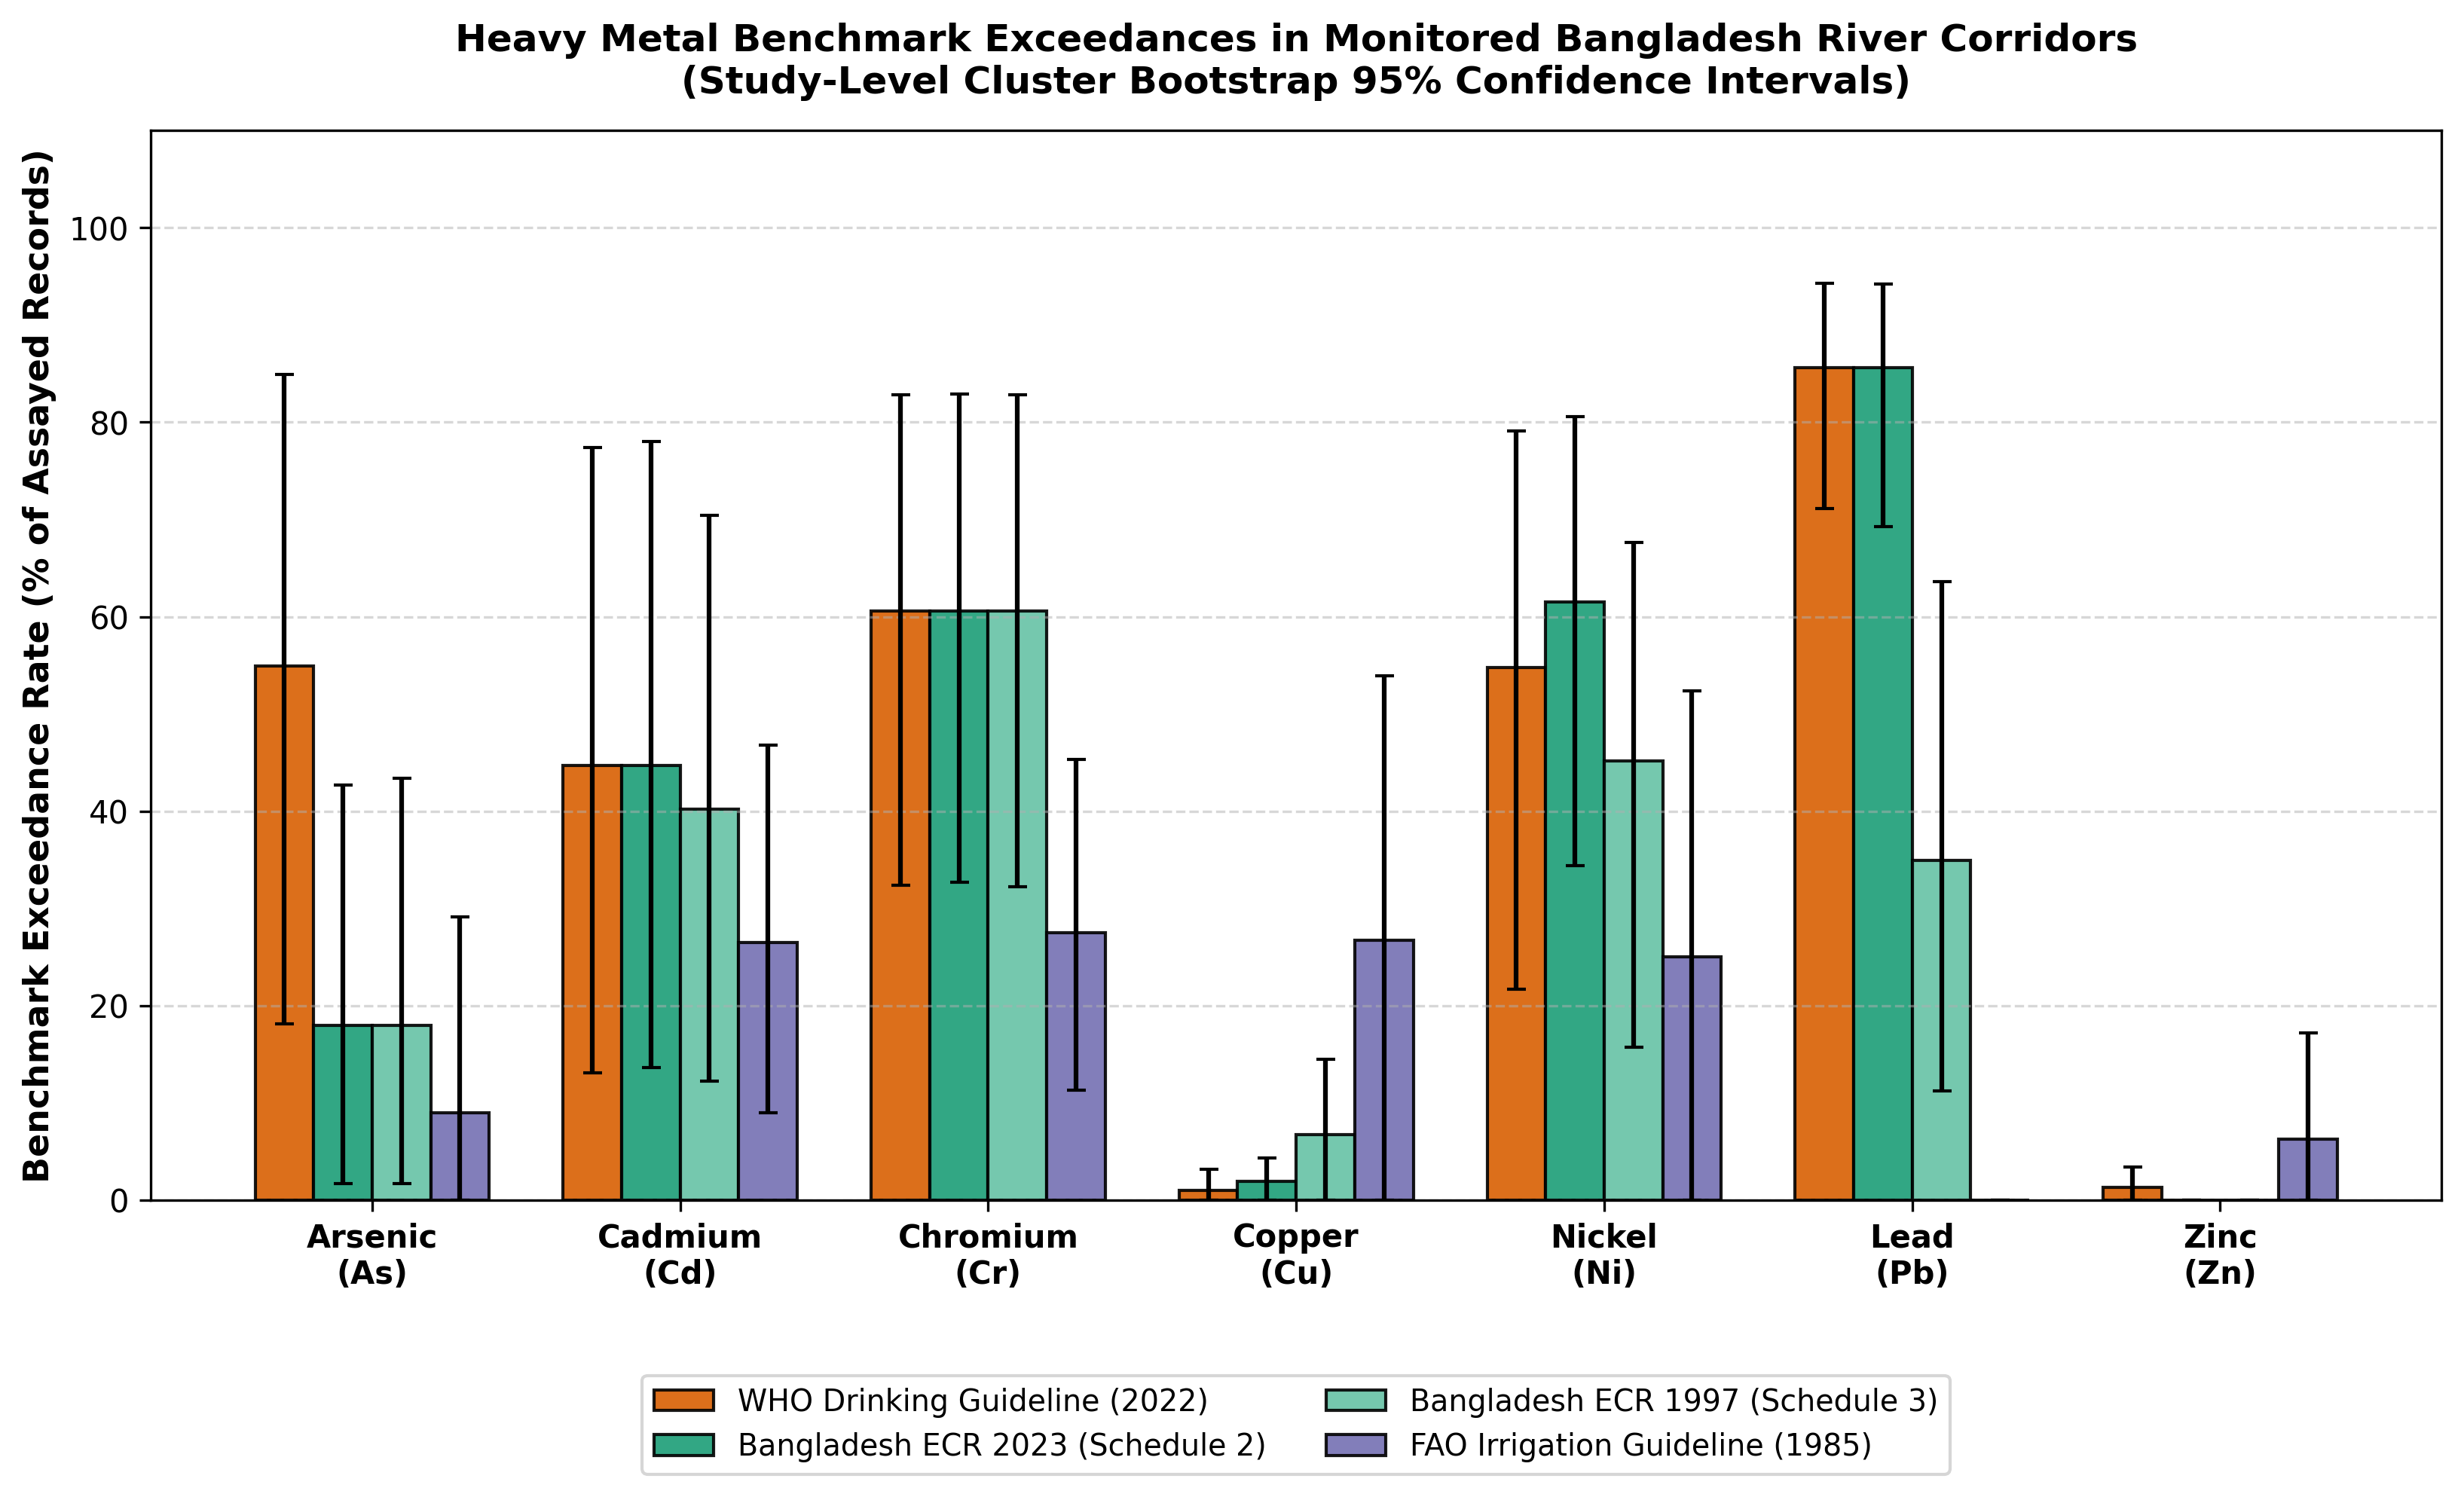
\includegraphics[width=0.98\textwidth]{fig1_exceedance.png}
\caption{Benchmark exceedance proportions of heavy metals in published Bangladesh river waters against WHO drinking guidelines, historical Bangladesh ECR 1997, contemporary ECR 2023, and FAO irrigation benchmarks, with error bars indicating 95\% study-level cluster bootstrap confidence intervals.}
\label{fig:exceedance}
\end{figure}

\subsection{Standardized Multi-Metal Pollution Indices (\texorpdfstring{$\mathrm{HPI}$, $\mathrm{HEI}$, $\mathrm{HQ}_{\mathrm{mean}}$}{HPI, HEI, HQmean})}
Evaluation of the standardized Core-4 fixed panel (As, Cd, Cr, Pb; $N=\HpiCoreFourN$) resolved index comparability across river systems (Table~\ref{tab:indices}):
\begin{itemize}
    \item \textbf{Core-4 $\mathrm{HPI}$ Distribution:} Across all 112 multi-metal records spanning 5 river systems and 7 studies, the median $\mathrm{HPI}$ was \textbf{\HpiCoreFourMedian} (Q1: \HpiCoreFourQOne, Q3: \HpiCoreFourQThree, IQR: \HpiCoreFourIqr, mean: \HpiCoreFourMean, maximum: \HpiCoreFourMax). Overall, \textbf{\HpiCoreFourShareAboveHundred\%} of records (66/112) exceeded Prasad and Bose's critical pollution threshold of 100, while \HpiCoreFourShareAboveTwoHundred\% exceeded 200.
    \item \textbf{Same-Subset Panel Evaluation (Resolving Sample Confounding):} Evaluating the effect of panel composition on the identical common subset ($N=35$; Supplementary Table~S3) revealed that median $\mathrm{HPI}$ remained virtually unchanged across Core-4 (\HpiCommonSubsetCoreFourMedian), Core-5 (\HpiCommonSubsetCoreFiveMedian), and All-7 (\HpiCommonSubsetAllSevenMedian), with all three panels exhibiting identical exceedance rates above the critical threshold (85.7\% $> 100$). Similarly, on the common $N=62$ subset, median $\mathrm{HPI}$ for Core-4 was 234.37 compared to 231.75 for Core-5 (both 74.2\% $> 100$). This demonstrates that expanding the metal panel produces negligible mathematical shift once sample composition is held constant (full-sample $N=112$ Core-4 median: \HpiCoreFourMedian), reflecting the structural damping of the Prasad and Bose inverse-standard weighting formula.
    \item \textbf{Linear Weights vs.\ Realized Score Contributions:} Numerator contribution analysis revealed that $\mathrm{HPI}$ is heavily dominated by Cadmium (median score contribution: 41.3\%) and Lead (35.8\%), followed by Arsenic (19.9\%), with Chromium contributing only 3.0\%. These realized scores closely reflect the quadratic scaling of inverse standards ($1/S_i^2$), whereas the linear unit weight shares ($W_i \propto 1/S_i$) are 60.2\% for Cd, 18.1\% for Pb, 18.1\% for As, and 3.6\% for Cr (Cd and Pb together account for 78.3\% of total linear weights, and 77.1\% of median index scores).
    \item \textbf{Concordance with $\mathrm{HEI}$ and Mean Hazard Quotient:} Across all records, Core-4 $\mathrm{HPI}$ and $\mathrm{HEI}$ exhibited strong monotonic rank agreement (Spearman $\rho = \HpiHeiSpearmanRho$, $p < 10^{-15}$). Across all Core-4 records, median $\mathrm{HEI}$ was \HeiMedian\ (mean: 23.47). Dividing by the four panel elements yields a median mean benchmark-normalized concentration ratio ($\mathrm{BCR}_{\mathrm{mean}} = \mathrm{HEI}/4$) of \MeanHqMedian, indicating that the median assayed water sample contains trace metals at approximately $1.7\times$ their individual WHO drinking guidelines.
    \item \textbf{River-Specific Variations:} Buriganga maintained the highest median $\mathrm{HPI}$ (1,977.43, $N=15$, 100\% $> 100$), followed by Karnaphuli (230.58, $N=20$, 100\% $> 100$) and Korotoa (195.00, $N=40$, 77.5\% $> 100$). Conversely, the southern deltaic rivers Kirtankhola (median: 57.06, $N=30$) and Rupsa (median: 52.51, $N=7$) showed 0.0\% exceedance of the critical $\mathrm{HPI}$ limit.
\end{itemize}

\begin{table}[htbp]
\centering
\small
\caption{Multi-metal pollution indices ($\mathrm{HPI}$, $\mathrm{HEI}$, $\mathrm{HQ}_{\mathrm{mean}}$) computed on the standardized Core-4 panel (As, Cd, Cr, Pb) across Bangladesh river systems.}
\label{tab:indices}
\begin{adjustbox}{width=\textwidth,center}
\begin{tabular}{lcccccccc}
\toprule
River System & $N$ & $k$ & Mean $\mathrm{HPI}$ & Median $\mathrm{HPI}$ & IQR $\mathrm{HPI}$ & $\%\, \mathrm{HPI} > 100$ & Median $\mathrm{HEI}$ & Mean $\mathrm{HQ}$ \\
\midrule
\textbf{Buriganga}$^\ddagger$ & 15 & 1 & 1,607.66 & 1,977.43 & 1,358.59 & 100.0\% & 51.60 & 12.90 \\
\textbf{Karnaphuli} & 20 & 1 & 253.70 & 230.58 & 133.47 & 100.0\% & 7.94 & 1.99 \\
\textbf{Korotoa} & 40 & 2 & 323.25 & 195.00 & 336.28 & 77.5\% & 10.20 & 2.55 \\
\textbf{Kirtankhola} & 30 & 1 & 60.21 & 57.06 & 42.05 & 0.0\% & 3.22 & 0.80 \\
\textbf{Rupsa} & 7 & 2 & 48.36 & 52.51 & 9.65 & 0.0\% & 1.97 & 0.49 \\
\midrule
\textbf{All Core-4 Records} & 112 & 7 & \textbf{\HpiCoreFourMean} & \textbf{\HpiCoreFourMedian} & \textbf{\HpiCoreFourIqr} & \textbf{\HpiCoreFourShareAboveHundred\%} & \HeiMedian & \MeanHqMedian \\
\bottomrule
\multicolumn{9}{l}{\footnotesize $^\ddagger$For the Buriganga River ($N=15$), the arithmetic mean $\mathrm{HPI}$ ($1,607.66$) is lower than the median ($1,977.43$) due to genuine negative skewness: 10 downstream} \\
\multicolumn{9}{l}{\footnotesize industrial stations cluster between $1,834$ and $2,458$, while two upstream reaches exhibit lower values ($\sim 258$), pulling the arithmetic mean downward.}
\end{tabular}
\end{adjustbox}
\end{table}

\subsection{Seasonal Contrast Dynamics: Pooled vs.\ Within-Study Contrasts}
Evaluating seasonal differences between winter dry-season and monsoon wet-season records revealed distinct element-specific behaviors (Table~\ref{tab:dilution}, Fig.~\ref{fig:dilution}):

\begin{table}[htbp]
\centering
\small
\caption{Seasonal comparison of heavy metal concentrations in Bangladesh rivers (Dry/Winter vs.\ Wet/Rainy season) with two-sided Mann-Whitney U tests, Holm-Bonferroni corrections, and within-study random-effects meta-analysis of study-level dry/wet ratios with Hartung-Knapp-Sidik-Jonkman (HKSJ) adjustment.}
\label{tab:dilution}
\begin{adjustbox}{width=\textwidth,center}
\begin{tabular}{lcccccccc|cccc}
\toprule
 & \multicolumn{8}{c|}{\textbf{Pooled Multi-Study Comparison}} & \multicolumn{4}{c}{\textbf{Within-Study Paired Meta-Analysis}} \\
Element & Dry $N$ & Dry Med & Wet $N$ & Wet Med & Ratio & $U$ & Two-Sided $p$ & Holm $p_{\mathrm{adj}}$ & $k_{\mathrm{pair}}$ & Pooled Ratio & DL 95\% CI & HKSJ 95\% CI \\
 & & (mg/L) & & (mg/L) & & & & & & & & \\
\midrule
\textbf{Arsenic (As)} & 57 & \ArsenicDryMedian & 23 & \ArsenicWetMedian & \textbf{\ArsenicDryWetRatio$\times$} & 927.5 & \textbf{\ArsenicTwoSidedP} & \textbf{\ArsenicHolmP$^*$} & 4 & \ArsenicWithinStudyRatio$\times$ & [0.83--2.44] & \ArsenicWithinStudyHksjCi \\
\textbf{Cadmium (Cd)} & 59 & 0.0015 & 27 & 0.0008 & 1.88$\times$ & 1,014.5 & 0.0429 & 0.2147 & 5 & 1.41$\times$ & [0.75--2.67] & [0.58--3.47] \\
\textbf{Chromium (Cr)} & 73 & 0.0710 & 28 & 0.0354 & 2.01$\times$ & 1,312.0 & 0.0281 & 0.1684 & 5 & 1.26$\times$ & [0.77--2.07] & [0.63--2.54] \\
\textbf{Lead (Pb)} & 67 & 0.0253 & 25 & 0.0287 & 0.88$\times$ & 859.0 & 0.8538 & 1.0000 & 4 & \LeadWithinStudyRatio$\times$ & [0.77--2.14] & \LeadWithinStudyHksjCi \\
\textbf{Zinc (Zn)} & 27 & 0.5300 & 17 & 0.0725 & 7.31$\times$ & 300.0 & 0.0915 & 0.3661 & 3 & 1.12$\times$ & [0.57--2.19] & [0.26--4.88] \\
\textbf{Nickel (Ni)} & 40 & 0.0685 & 18 & 0.0945 & 0.73$\times$ & 376.5 & 0.7880 & 1.0000 & 4 & 1.00$\times$ & [0.52--1.91] & [0.35--2.86] \\
\textbf{Copper (Cu)} & 40 & 0.0866 & 16 & 0.0571 & 1.52$\times$ & 391.0 & 0.2009 & 0.6027 & 4 & 0.54$\times$ & [0.11--2.50] & [0.04--6.53] \\
\bottomrule
\multicolumn{13}{l}{\footnotesize $^*$Statistically significant in pooled unclustered test after Holm-Bonferroni adjustment ($\alpha = 0.05$). DL: DerSimonian-Laird; HKSJ: Hartung-Knapp-Sidik-Jonkman small-sample adjustment.}
\end{tabular}
\end{adjustbox}
\end{table}

Key findings:
\begin{itemize}
    \item \textbf{Simpson's Paradox and Statistical Power under Small-Sample Adjustments ($k=3\text{--}5$):} In the pooled multi-study dataset, Lead and Nickel appeared slightly higher in the wet season (pooled dry/wet ratios of 0.88$\times$ for Pb and 0.73$\times$ for Ni). However, cross-study pooled comparisons risk spatial confounding if studies contributing wet-season samples are located predominantly in contaminated corridors. When controlling for station geography using within-study paired meta-analyses across matched stations, point ratios indicate dry-season enrichment (\LeadWithinStudyRatio$\times$ for Pb, \ArsenicWithinStudyRatio$\times$ for As, 1.41$\times$ for Cd, 1.26$\times$ for Cr, and 1.00$\times$ for Ni). Nevertheless, applying the Hartung-Knapp-Sidik-Jonkman (HKSJ) adjustment to account for small paired study counts ($k=3\text{--}5$) yields wide 95\% confidence intervals that span unity across all seven metals (Pb: \LeadWithinStudyHksjCi; As: \ArsenicWithinStudyHksjCi; Ni: [0.35--2.86]; Cr: [0.63--2.54]; Cd: [0.58--3.47]; Cu: [0.04--6.53]; Zn: [0.26--4.88]). Because the pooled ratios (0.88$\times$ for Pb and 0.73$\times$ for Ni) fall well within these wide HKSJ intervals, the pooled and within-study estimates are statistically indistinguishable, and within-study seasonal variations cannot be declared statistically significant given current literature limitations.
    \item \textbf{Tripartite Arsenic Hydrological Distribution:} Comparing Table~\ref{tab:exceedance} and Table~\ref{tab:dilution} reveals that both dry-season (\ArsenicDryMedian~mg/L, $N=57$) and wet-season (\ArsenicWetMedian~mg/L, $N=23$) Arsenic medians are lower than the overall pooled median of \ArsenicOverallMedian~mg/L ($N=122$). This divergence is explained by the 41 pre-monsoon summer records (March to May; median: \textbf{\ArsenicPremonsoonMedian~mg/L}, mean: \ArsenicPremonsoonMean~mg/L). Pre-monsoon conditions represent the annual hydrochemical maximum due to lowest baseflow, elevated evaporative concentration, and intensive pumping of shallow alluvial aquifers during boro rice irrigation. Excluding these pre-monsoon peak observations from the binary dry (winter) vs.\ wet (monsoon) contrast lowers both seasonal medians relative to the pooled annual dataset.
\end{itemize}

\begin{figure}[htbp]
\centering
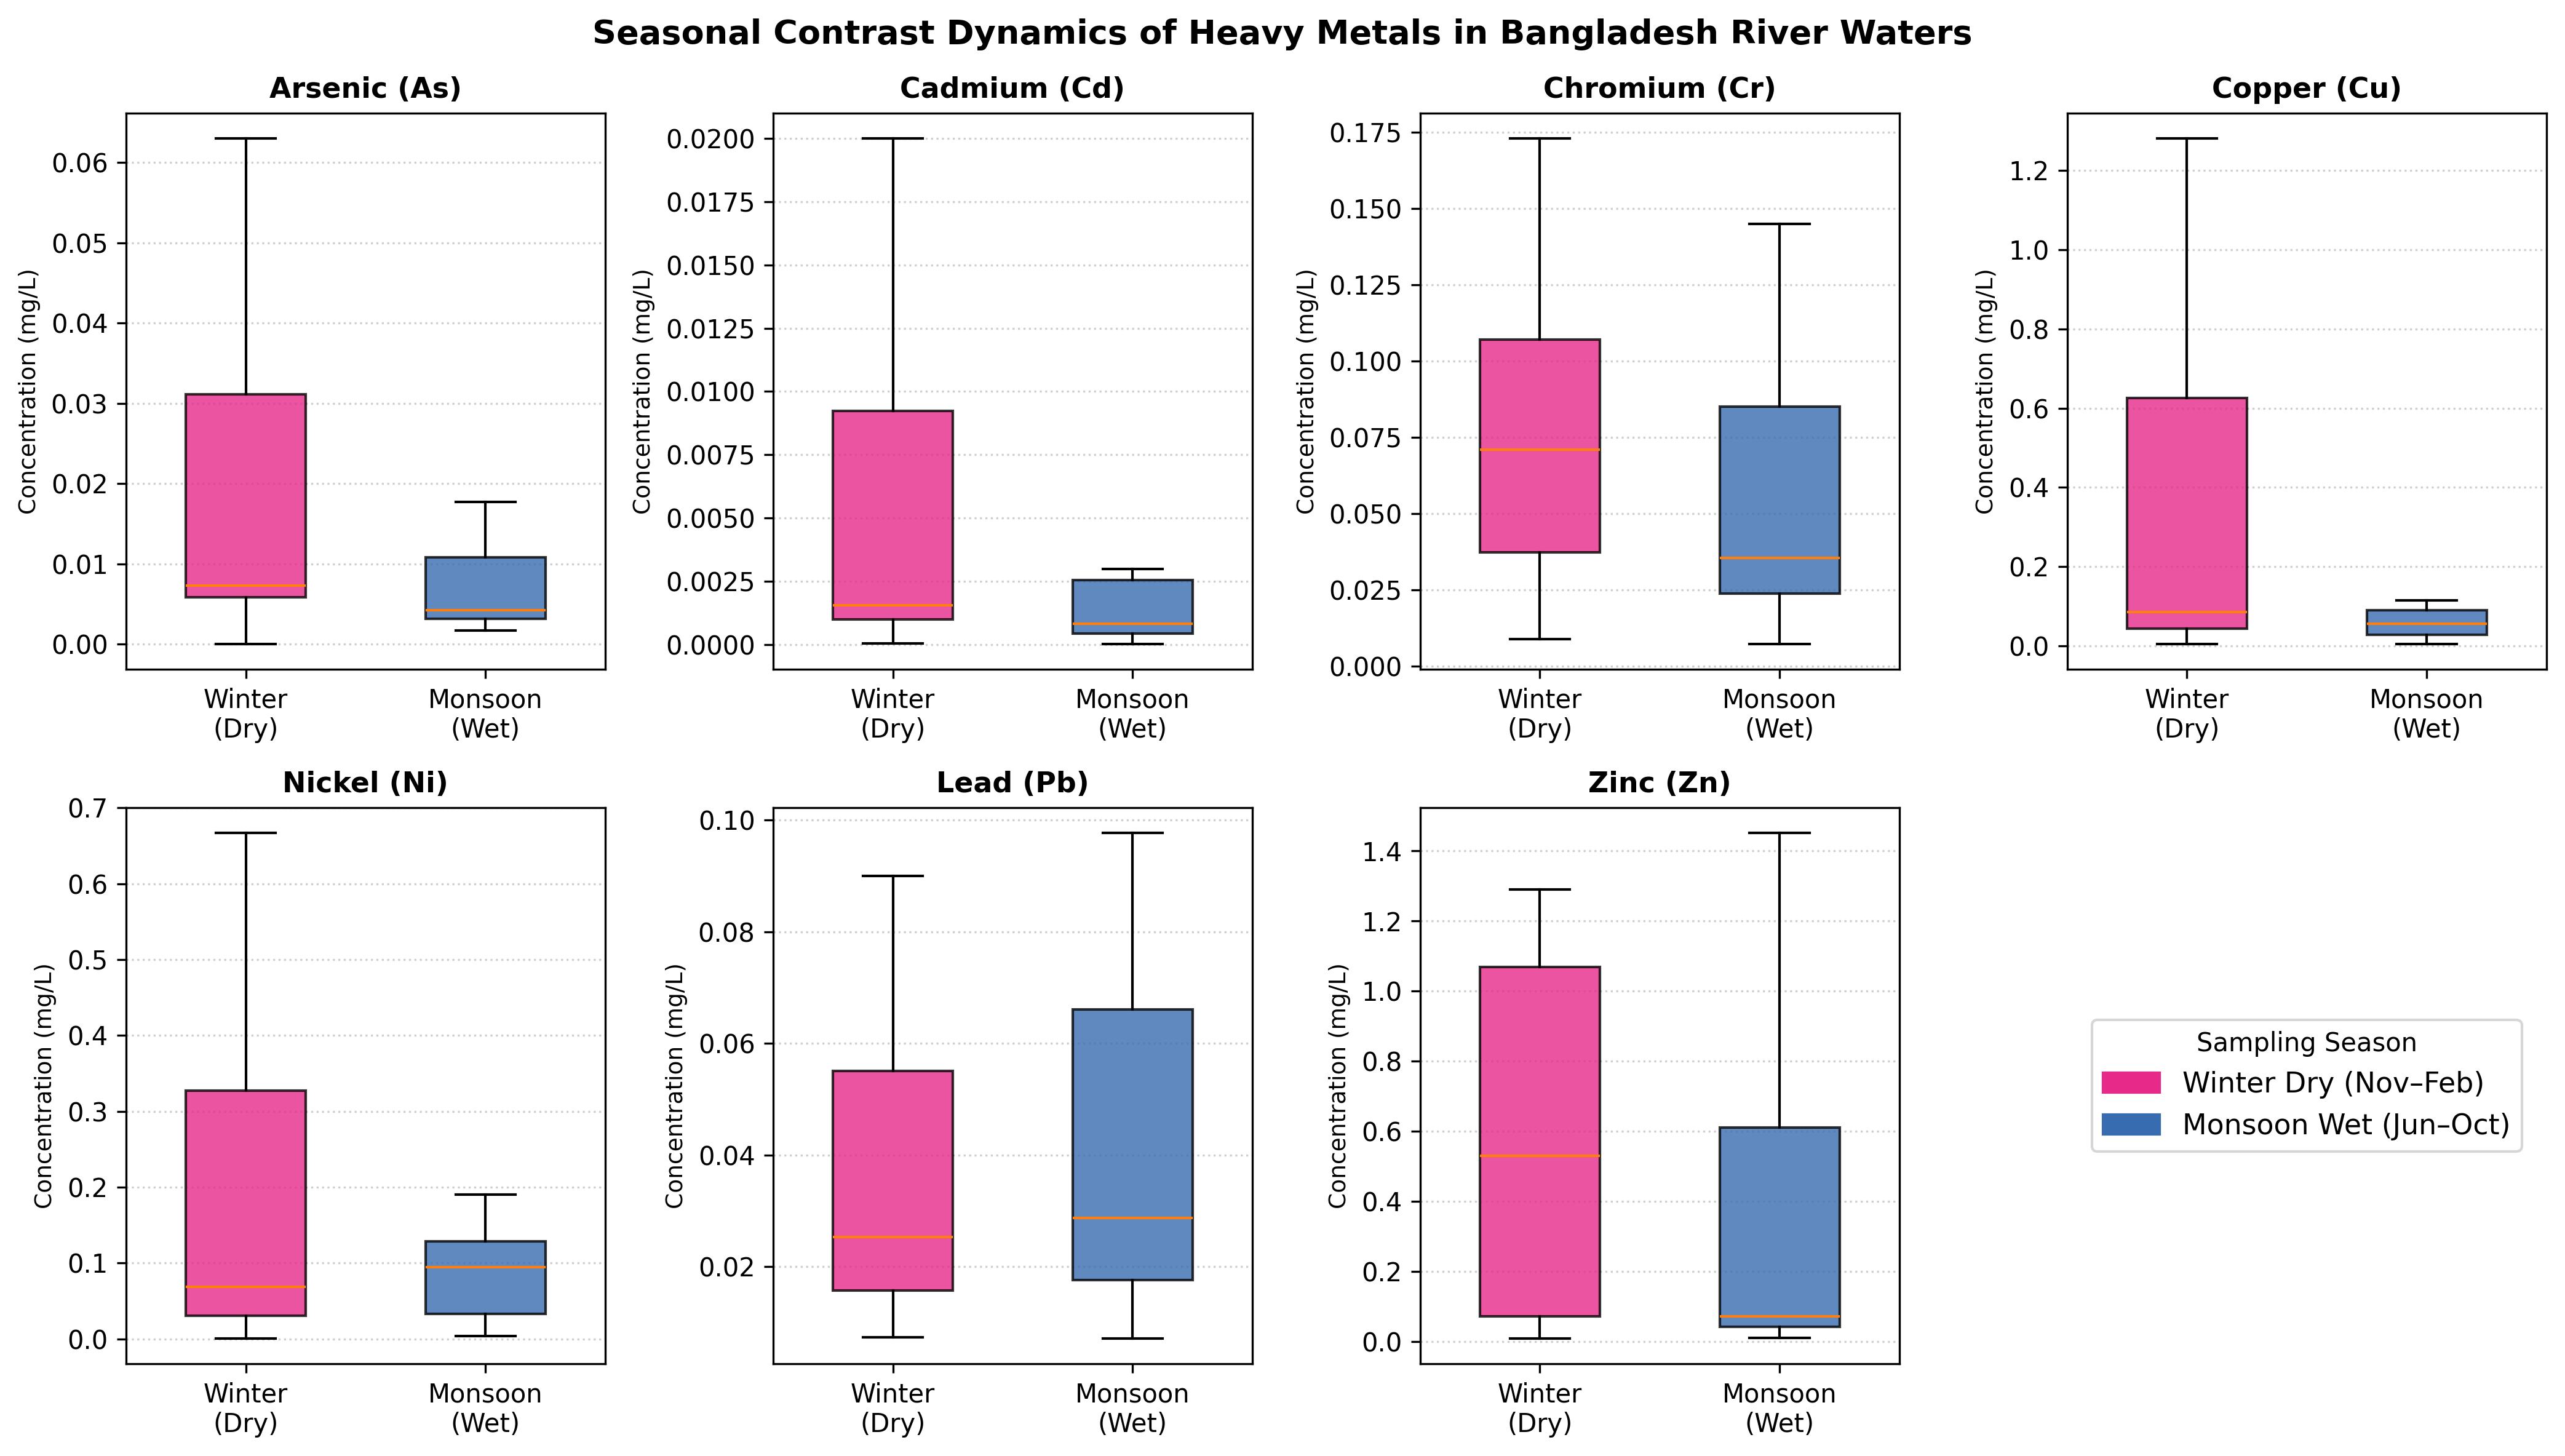
\includegraphics[width=0.98\textwidth]{fig2_dilution.png}
\caption{Seasonal concentration distributions (Winter Dry vs.\ Monsoon Wet) across seven heavy metals (As, Cd, Cr, Cu, Ni, Pb, Zn) in Bangladesh river waters. Center line indicates median, box bounds denote interquartile range (IQR, 25th--75th percentiles), and whiskers extend to $1.5\times\mathrm{IQR}$ (extreme outliers suppressed for visual clarity; maximum concentrations reported in Table~\ref{tab:exceedance}).}
\label{fig:dilution}
\end{figure}

\subsection{River Network Coverage and Spatial Null Model}
Spatial analysis across HydroSHEDS HydroRIVERS strictly within Bangladesh territory demonstrated that compiled academic literature covers only a small fraction of the primary river network (Table~\ref{tab:spatial_summary}, Fig.~\ref{fig:spatial_map}):
\begin{itemize}
    \item \textbf{Network-Wide Coverage Gaps in Compiled Literature:} Across \TotalMajorReachesCount\ major river reach segments (Strahler order $\ge 4$, mean discharge $Q \ge 50\text{ m}^3/\text{s}$) strictly within Bangladesh territory (totaling \TotalMajorLengthKm~km), \textbf{\UnsampledCountTwentyFiveKm\ reaches (\UnsampledPctCountTwentyFiveKm\% by count)} totaling \textbf{\UnsampledLengthTwentyFiveKm~km (\UnsampledPctLengthTwentyFiveKm\% by length)} lie more than 25~km straight-line from any published sampling point (\UniqueStationCoordinates\ unique coordinate locations cataloged in the audit corpus).
    \item \textbf{Topological Along-Network Distance:} When evaluated along stream network topology using Dijkstra's algorithm, the uncovered proportion rises to \textbf{\UnsampledPctLengthNetworkTwentyFiveKm\%} of major reach length (4,094.5~km) at the 25~km network threshold, confirming that straight-line Euclidean distance overestimates true riverine surveillance coverage.
    \item \textbf{Spatial Monte Carlo Null Model:} Under 1,000 Monte Carlo simulations placing \UniqueStationCoordinates\ random stations along the national major river network, expected coverage at 25~km was \NullModelMeanCoveragePct\% (95\% CI: [\NullModelCiLoPct\%--\NullModelCiHiPct\%]). The observed coverage of \ObservedCoveredPct\% (\ObservedCoveredLengthKm~km) is significantly lower than random expectation ($p \NullModelPvalFormatted$), demonstrating that compiled academic literature is clustered around accessible urban-industrial centers and port facilities. Because the 23 published coordinates represent approximately 10 distinct study reach sectors, study-level clustering contributes substantially to this localized footprint.
\end{itemize}

\begin{table}[htbp]
\centering
\small
\caption{Spatial coverage evaluation of compiled water quality studies across major Bangladesh river channels (\TotalMajorReachesCount\ reaches totaling \TotalMajorLengthKm~km strictly in Bangladesh) evaluated under straight-line (Haversine) and along-network topological stream distances.}
\label{tab:spatial_summary}
\begin{adjustbox}{width=\textwidth,center}
\begin{tabular}{lcccc}
\toprule
Metric & Unsampled Reaches & Pct Reaches (\%) & Unsampled Length (km) & Pct Length (\%) \\
\midrule
Straight-Line (Haversine) $>10$~km & 2,126 & 95.6\% & 4,379.7 & \UnsampledPctLengthTenKm\% \\
Straight-Line (Haversine) $>25$~km & \UnsampledCountTwentyFiveKm & \UnsampledPctCountTwentyFiveKm\% & \UnsampledLengthTwentyFiveKm & \textbf{\UnsampledPctLengthTwentyFiveKm\%} \\
Straight-Line (Haversine) $>50$~km & 1,432 & 64.4\% & 2,732.0 & \UnsampledPctLengthFiftyKm\% \\
Along-Network Stream Distance $>25$~km & 2,058 & 92.5\% & 4,094.5 & \textbf{\UnsampledPctLengthNetworkTwentyFiveKm\%} \\
\bottomrule
\end{tabular}
\end{adjustbox}
\end{table}

\begin{figure}[htbp]
\centering
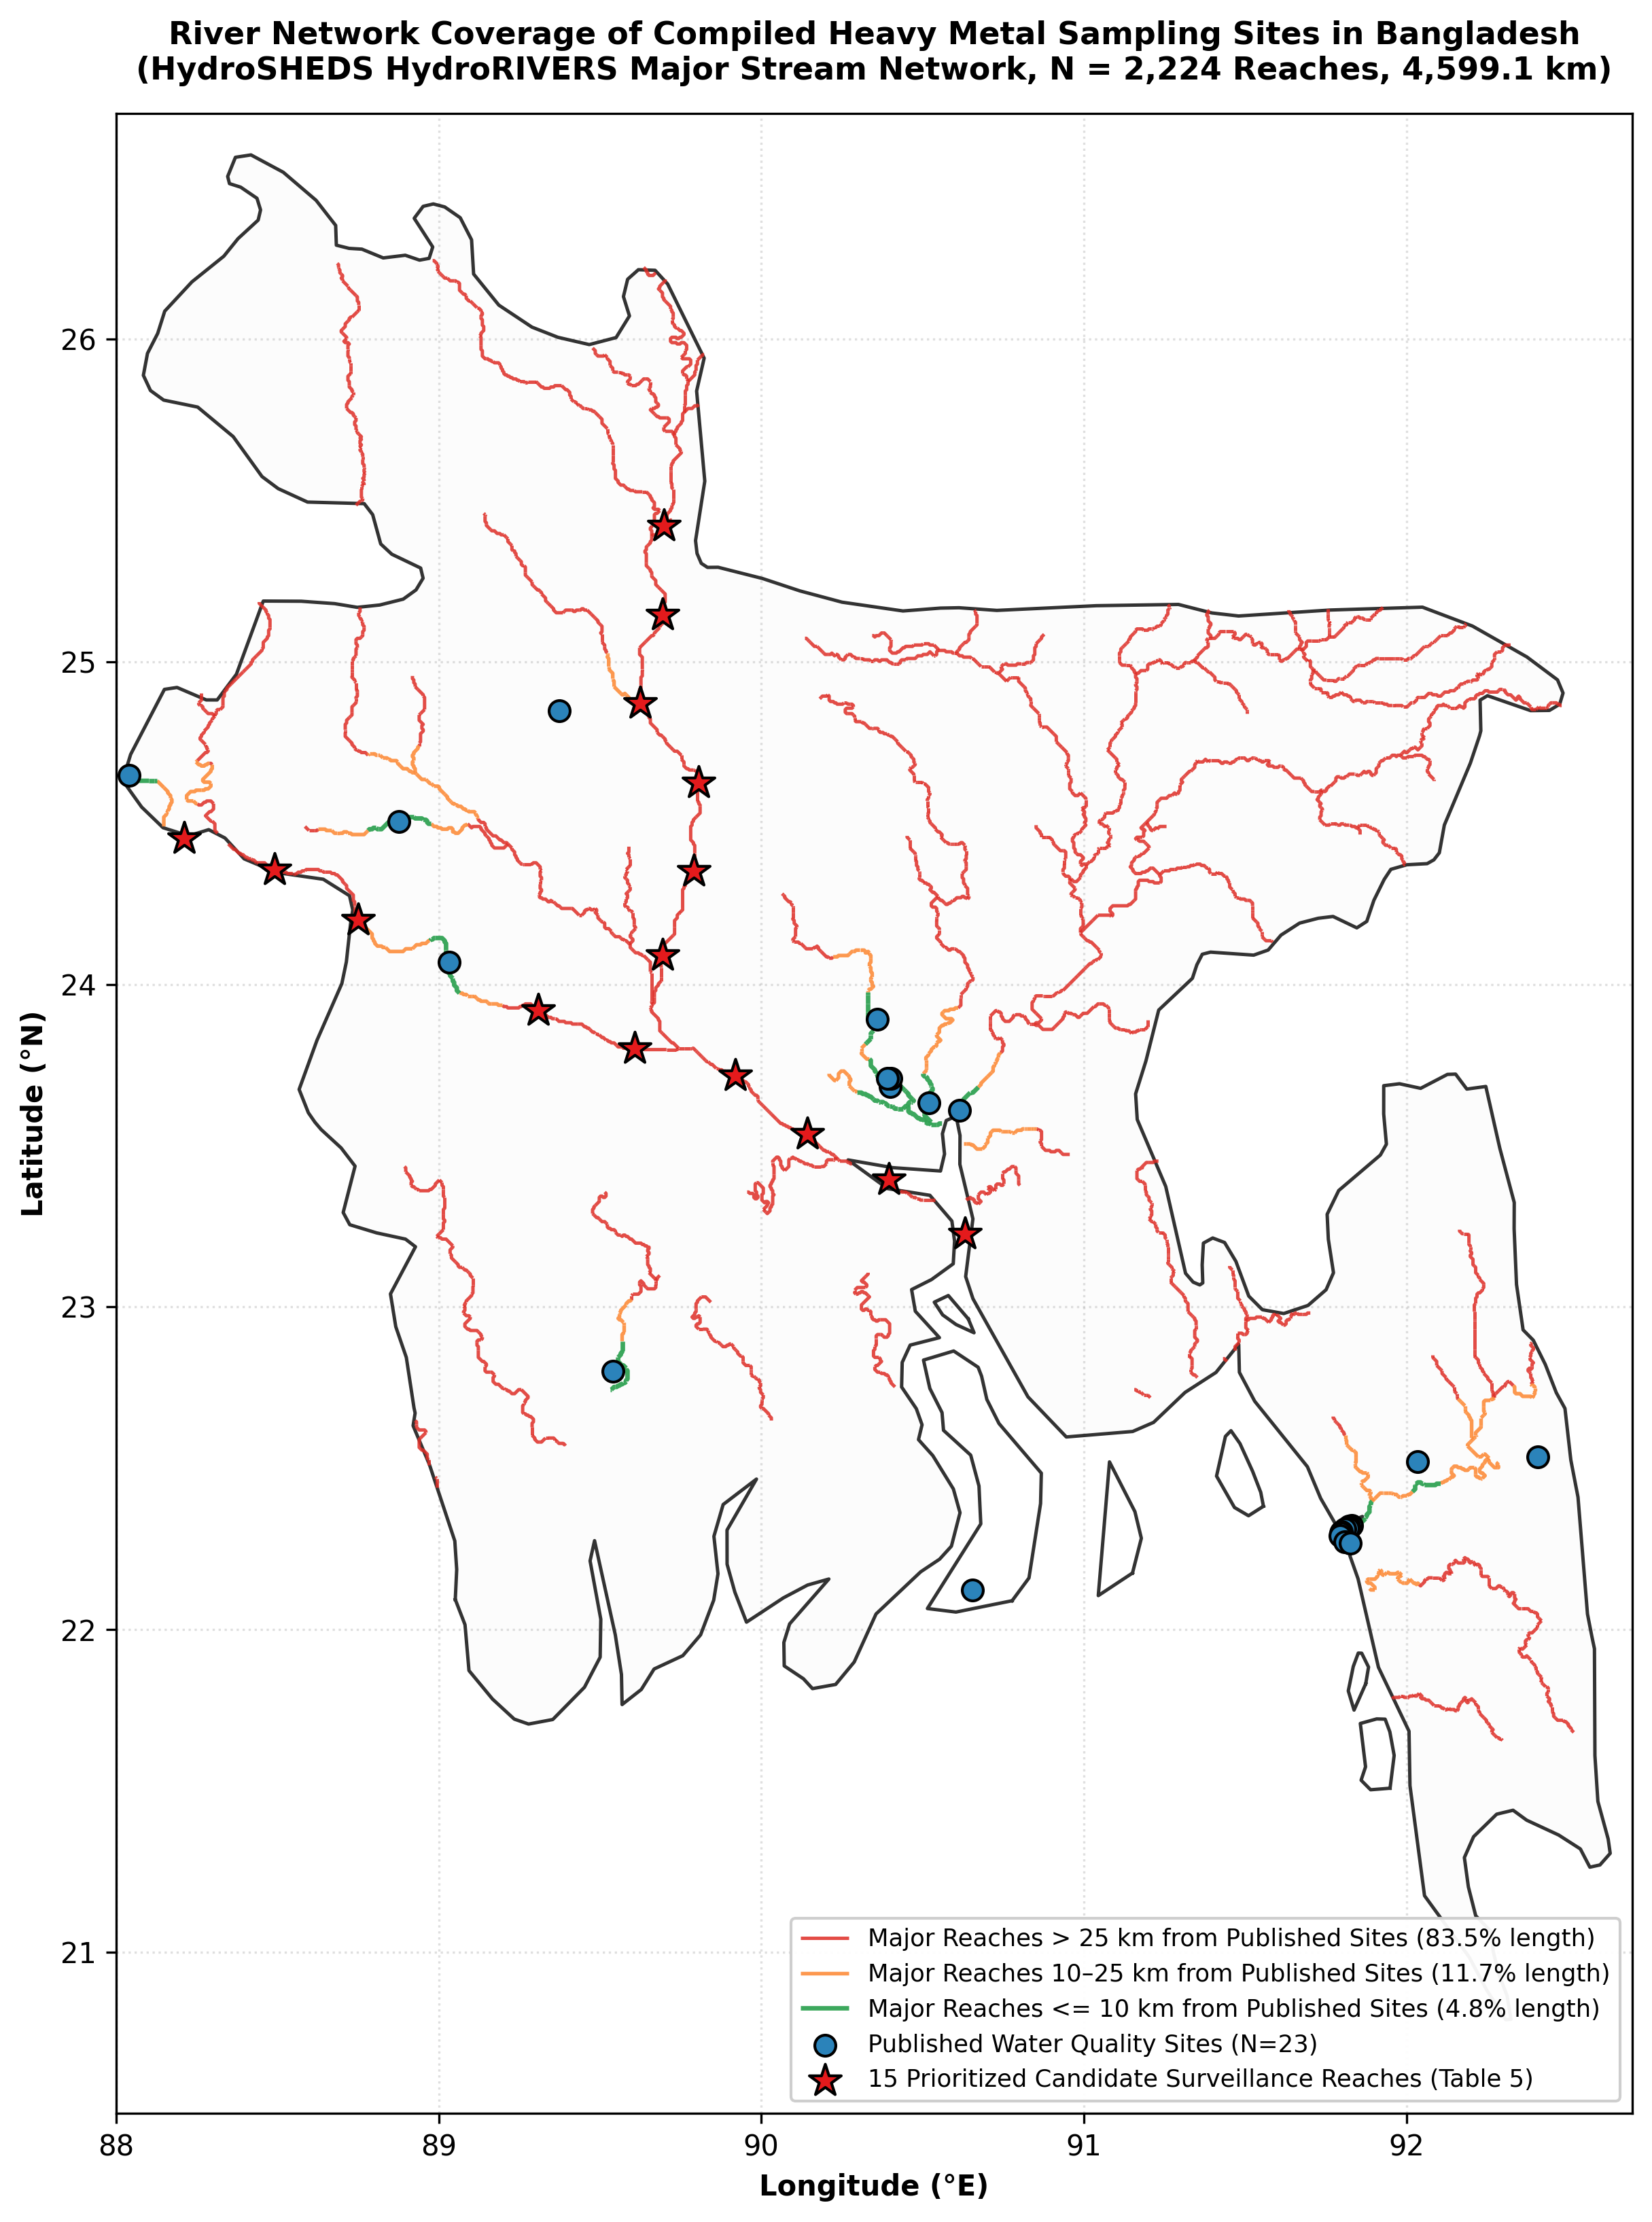
\includegraphics[width=0.82\textwidth]{fig3_spatial_coverage_map.png}
\caption{Spatial coverage of compiled published water quality sampling sites in Bangladesh and unsampled major river reaches ($>25$~km straight-line distance), strictly clipped to the Bangladesh national boundary outline, showing the 23 published sampling sites (blue circles) and 15 geographically diverse candidate monitoring reaches (red stars, Table~\ref{tab:stations}).}
\label{fig:spatial_map}
\end{figure}

To address these gaps, 15 geographically diverse candidate monitoring reaches in unstudied river sectors were identified (Table~\ref{tab:stations}), enforcing $\ge 30$~km spatial separation and verifying administrative names against gazetteers.

\begin{table}[htbp]
\centering
\small
\caption{Candidate river reaches in unsampled sectors ($>25$~km from published sites) prioritized by catchment area, enforcing $\ge 30$~km spatial separation with gazetteer-verified administrative reach names.}
\label{tab:stations}
\begin{adjustbox}{width=\textwidth,center}
\begin{tabular}{clcccccl}
\toprule
Rank & Candidate ID & Lat ($^\circ$N) & Lon ($^\circ$E) & Order & Catchment ($\text{km}^2$) & Dist.\ to Published Site (km) & Target River Reach (Gazetteer Verified) \\
\midrule
1 & \texttt{GAP\_STN\_01}$^\dagger$ & 23.227 & 90.631 & 9 & 1,574,223 & 42.6 & Lower Meghna Mainstem (Chandpur--Haimchar Confluence Reach) \\
2 & \texttt{GAP\_STN\_02} & 23.395 & 90.395 & 9 & 1,488,391 & 29.3 & Padma--Meghna Estuarine Convergence (Munshiganj Reach) \\
3 & \texttt{GAP\_STN\_03} & 23.535 & 90.144 & 9 & 1,485,761 & 30.9 & Lower Padma Main Channel (Jazira--Louhajang Reach, Shariatpur/Munshiganj) \\
4 & \texttt{GAP\_STN\_04} & 23.718 & 89.919 & 9 & 1,485,272 & 48.2 & Upper Padma Mainstem (Goalundo Reach, Rajbari) \\
5 & \texttt{GAP\_STN\_05} & 23.802 & 89.608 & 8 & 944,490 & 65.6 & Ganges--Jamuna Convergence Reach (Pangsha--Sujanagar, Rajbari/Pabna) \\
6 & \texttt{GAP\_STN\_06} & 23.919 & 89.309 & 8 & 943,786 & 32.6 & Upper Ganges Mainstem (Kumarkhali--Ishwardi Reach, Kushtia/Pabna) \\
7 & \texttt{GAP\_STN\_07} & 24.200 & 88.750 & 8 & 942,749 & 32.2 & Central Ganges Channel (Charghat--Bagha Reach, Rajshahi/Natore) \\
8 & \texttt{GAP\_STN\_08} & 24.356 & 88.492 & 8 & 941,812 & 42.3 & North-West Padma Reach (Rajshahi Sadar Upstream) \\
9 & \texttt{GAP\_STN\_09} & 24.452 & 88.210 & 8 & 929,834 & 27.9 & Upper Border Ganges Reach (Shibganj, Chapai Nawabganj) \\
10 & \texttt{GAP\_STN\_10} & 24.089 & 89.695 & 8 & 521,878 & 67.2 & Lower Jamuna Channel (Chauhali--Tangail Reach, Sirajganj/Tangail) \\
11 & \texttt{GAP\_STN\_11} & 24.351 & 89.790 & 8 & 520,951 & 69.6 & Central Jamuna Mainstem (Belkuchi Reach, Sirajganj--Tangail) \\
12 & \texttt{GAP\_STN\_12} & 24.624 & 89.805 & 8 & 520,682 & 50.3 & Upper Jamuna Channel (Bhuapur--Sirajganj Reach) \\
13 & \texttt{GAP\_STN\_13} & 24.872 & 89.624 & 8 & 514,663 & 25.5 & Jamuna Confluence (Kazipur--Sariakandi Reach, Bogura) \\
14 & \texttt{GAP\_STN\_14} & 25.146 & 89.694 & 8 & 514,278 & 46.2 & Brahmaputra Mainstem (Fulchhari--Dewanganj Reach, Gaibandha/Jamalpur) \\
15 & \texttt{GAP\_STN\_15} & 25.421 & 89.698 & 8 & 500,939 & 71.5 & Upper Brahmaputra Entry Reach (Chilmari, Kurigram) \\
\bottomrule
\multicolumn{8}{l}{\footnotesize "Dist.\ to Published Site" measures straight-line distance to the nearest historical sampling location (all $>25$~km by design).} \\
\multicolumn{8}{l}{\footnotesize Candidate reaches were prioritized by upstream catchment area while enforcing $\ge 30$~km spatial separation along major channels.} \\
\multicolumn{8}{l}{\footnotesize $^\dagger$Candidate reaches in wide, dynamic estuarine channels (e.g., \texttt{GAP\_STN\_01}, Chandpur confluence, $>2$~km wide) represent incomplete cross-sectional mixing zones;} \\
\multicolumn{8}{l}{\footnotesize monitoring requires depth-integrated, multi-point cross-channel transects across ebb and flood tidal phases rather than single unrepresentative grab samples.} \\
\end{tabular}
\end{adjustbox}
\end{table}

\section{Discussion}

\subsection{Regulatory Benchmark Discordance: Potable Screening and ECR 2023 Standards}
Our multi-study synthesis evaluates heavy metal concentrations in Bangladesh river waters against evolving national and international regulatory frameworks. Ambient river water is raw surface water rather than finished tap water; therefore, screening river concentrations against potable criteria serves to assess ambient chemical pressure and the coagulation/purification challenge imposed on municipal water treatment plants abstracting surface waters. Under the historical Environmental Conservation Rules \citep{ECR1997}, national potable limits were substantially more lenient than international health benchmarks: Lead exceedance was \LeadBdNineteenNinetySevenExceedPct\% (vs.\ \LeadWhoExceedPct\% under WHO), Cadmium was \CadmiumBdNineteenNinetySevenExceedPct\% (vs.\ \CadmiumWhoExceedPct\% WHO), and Nickel was \NickelBdNineteenNinetySevenExceedPct\% (vs.\ \NickelWhoExceedPct\% WHO). 

However, with the gazetting of the Environmental Conservation Rules 2023 (ECR 2023 Schedule 2; S.R.O. 53-Law/2023), the Government of Bangladesh officially repealed ECR 1997 and adopted substantially stricter potable thresholds. By lowering the national Lead standard from 0.050 to 0.010~mg/L (matching the WHO guideline), exceedance in published river water records rises from \LeadBdNineteenNinetySevenExceedPct\% to \textbf{\LeadBdTwentyTwentyThreeExceedPct\%}, eliminating the historical divergence between international and domestic benchmarks. Similarly, tightening Cadmium from 0.005 to 0.003~mg/L raises exceedance to \textbf{\CadmiumBdTwentyTwentyThreeExceedPct\%}, while tightening Nickel from 0.100 to 0.050~mg/L (stricter than WHO's 0.070~mg/L guideline) increases national benchmark exceedance to \textbf{\NickelBdTwentyTwentyThreeExceedPct\%}. Consequently, earlier literature concluding that Bangladeshi rivers generally conformed to national statutory limits relied on an obsolete regulatory baseline. Under current national standards, monitored surface water corridors exhibit extensive chemical pressure.

\subsection{Operational Fraction Confounding: Dissolved vs.\ Total Digestions}
A paramount methodological challenge in synthesizing fluvial trace elements in the Bengal Delta is distinguishing between dissolved and suspended particulate metal fractions. The Ganges-Brahmaputra-Meghna system transports over one billion metric tons of suspended sediment annually, with riverine suspended sediment concentrations frequently exceeding 500 to 2,000~mg/L during peak monsoonal runoff \citep{Goodbred1999}. Because trace elements such as Pb, Cr, and Fe possess high solid-water partition coefficients ($\log K_d \approx 4\text{--}6\text{ L/kg}$), digesting whole, unfiltered water captures vast quantities of particulate-bound lattice minerals, inflating apparent water concentrations by one to three orders of magnitude above the dissolved phase \citep{Gaillardet2014}.

In our compiled dataset, 10 investigations explicitly reported filtering water samples through 0.45~$\mu\text{m}$ membrane filters followed by preservation with nitric acid (Supplementary Table~S1), while two studies did not document filtration. Crucially, when we restricted our sensitivity analysis strictly to confirmed dissolved records ($k=10$ studies, $N=131$--$139$), WHO exceedance proportions remained exceptionally high: \textbf{\LeadConfirmedDissolvedWhoPct\%} for Lead, \textbf{\ChromiumConfirmedDissolvedWhoPct\%} for Chromium, \textbf{\ArsenicConfirmedDissolvedWhoPct\%} for Arsenic, and \textbf{\CadmiumConfirmedDissolvedWhoPct\%} for Cadmium. Comparing dissolved medians from confirmed filtered studies—Lead (\LeadConfirmedDissolvedMedian~mg/L), Chromium (\ChromiumConfirmedDissolvedMedian~mg/L), Nickel (\NickelConfirmedDissolvedMedian~mg/L), Arsenic (\ArsenicConfirmedDissolvedMedian~mg/L), and Cadmium (\CadmiumConfirmedDissolvedMedian~mg/L)—against Gaillardet et al.'s (2014) global baseline for unpolluted major rivers ($0.05\text{--}2.0~\mu\text{g/L}$ for Pb; $0.5\text{--}2.0~\mu\text{g/L}$ for Cr) confirms that published concentrations in monitored corridors are enriched in the dissolved phase by one to two orders of magnitude above unpolluted global baselines.

Furthermore, the instrument stratification analysis (Table~S1) directly addresses concerns regarding whether high flame-AAS detection limits inflate exceedance estimates. In investigations employing high-sensitivity spectrometry with detection limits $<0.001$~mg/L (GF-AAS, HG-AAS, ICP-MS; $N=\LeadHighSensN, k=\LeadHighSensK$), \textbf{\LeadHighSensExceedPct\%} of records still exceeded the WHO Lead guideline (median: \LeadHighSensMedian~mg/L). This demonstrates that elevated Lead concentrations and guideline exceedances are characteristic of measurements performed on high-sensitivity instruments with detection limits well below the 0.010~mg/L threshold, confirming that observed exceedances cannot be attributed to flame-AAS detection limit artifacts.

\subsection{Mathematical Artifacts in the Heavy Metal Pollution Index (\texorpdfstring{$\mathrm{HPI}$}{HPI})}
Our evaluation resolves a widespread misconception in published environmental index literature regarding panel invariance. When standardizing the $\mathrm{HPI}$ across identical subsets ($N=35$), median $\mathrm{HPI}$ remained virtually unchanged across Core-4 (\HpiCommonSubsetCoreFourMedian), Core-5 (\HpiCommonSubsetCoreFiveMedian), and All-7 (\HpiCommonSubsetAllSevenMedian). Rather than demonstrating ecological stability, this behavior is a direct mathematical consequence of Prasad and Bose's \citeyearpar{Prasad2001} formulation. Because $Q_i = (M_i / S_i) \times 100$ and $W_i \propto 1/S_i$, the numerator scales quadratically as $\sum M_i / S_i^2$. Squaring the inverse standard magnifies the disparity between Cadmium ($1/0.003^2 = 1.11 \times 10^5$) and Zinc ($1/3.0^2 = 0.11$) by a factor of $1.0 \times 10^6$ (one million to one). As a result, Cadmium and Lead account for \textbf{60.2\%} and \textbf{18.1\%} of the total Core-4 linear weight (summing to \textbf{\HpiCdPbWeightSharePct\%}), and 41.3\% and 35.8\% of realized median index scores (summing to 77.1\%). Conversely, elements with higher limits such as Copper ($S=2.0\text{ mg/L}$, $1/S^2 = 0.25$) and Zinc ($S=3.0\text{ mg/L}$, $1/S^2 = 0.11$) contribute negligibly to the weighted score. Structurally, $\mathrm{HPI}$ is an ill-conditioned proxy for Cadmium and Lead. We therefore recommend complementing $\mathrm{HPI}$ with linear unweighted metrics such as the Heavy Metal Evaluation Index ($\mathrm{HEI}$, median: \HeiMedian, equivalent to $\mathrm{MI}$) and the mean hazard quotient ($\mathrm{HQ}_{\mathrm{mean}} = \mathrm{HEI}/4 = \MeanHqMedian$), which assign equal diagnostic value to all audited contaminants.

\subsection{Seasonal Dynamics, Tripartite Arsenic Partition, and Meta-Analytic Power}
Evaluating seasonal variations revealed important methodological distinctions between pooled and within-study estimators. In pooled multi-study comparisons, Lead and Nickel appeared slightly higher in the monsoon wet season (pooled ratios 0.88$\times$ and 0.73$\times$). However, cross-study pooled comparisons risk spatial confounding if wet-season sampling was conducted predominantly in heavily contaminated industrial corridors. In paired within-study meta-analyses across matched stations, point ratios consistently indicate dry-season enrichment (\LeadWithinStudyRatio$\times$ for Pb, \ArsenicWithinStudyRatio$\times$ for As, 1.41$\times$ for Cd, 1.26$\times$ for Cr, and 1.00$\times$ for Ni).

Crucially, our application of the Hartung-Knapp-Sidik-Jonkman (HKSJ) adjustment to paired meta-analyses ($k=3\text{--}5$) widens 95\% confidence intervals (Pb: \LeadWithinStudyHksjCi; As: \ArsenicWithinStudyHksjCi; Ni: [0.35--2.86]; Cr: [0.63--2.54]; Cd: [0.58--3.47]; Cu: [0.04--6.53]; Zn: [0.26--4.88]). Because all HKSJ intervals span unity, and because pooled ratios fall well within these bounds, within-study seasonal variations cannot be declared statistically significant with small paired study numbers, frankly reflecting statistical power limitations in published literature.

Furthermore, our sample accounting clarifies the apparent discrepancy where both dry-season (\ArsenicDryMedian~mg/L) and wet-season (\ArsenicWetMedian~mg/L) Arsenic medians were lower than the pooled overall median (\ArsenicOverallMedian~mg/L). Pre-monsoon summer records ($N=\ArsenicPremonsoonN$, median: \textbf{\ArsenicPremonsoonMedian~mg/L}, mean: \ArsenicPremonsoonMean~mg/L) represent the annual concentration peak. During this period, river baseflow reaches its annual minimum, ambient temperatures maximize evaporative concentration, and intensive boro rice irrigation abstracts large volumes of shallow alluvial groundwater \citep{Brammer2009,Halim2015}. Excluding this pre-monsoon peak from binary dry (winter) vs.\ wet (monsoon) contrasts lowers both seasonal medians relative to the annual pooled dataset.

\subsection{Geographical Representativeness and Academic Spatial Bias}
The Core-4 multi-metal index is derived from 5 river systems across 7 studies ($N=112$), in which three industrial corridors—Buriganga ($N=15$), Korotoa ($N=40$), and Karnaphuli ($N=20$)—account for 67\% of all observations. These reaches receive continuous discharges from tannery estates, textile dyeing mills, and industrial clusters. Our HydroSHEDS network analysis demonstrates that \UnsampledPctLengthTwentyFiveKm\% of major river reach length (3,841.9~km across 1,890 segments) has zero published academic monitoring within 25~km in the audited corpus. The spatial Monte Carlo null model ($p \NullModelPvalFormatted$) confirms extreme clustering around accessible urban-industrial hubs. While broader multi-decade compilations (e.g., \citealt{Bilal2023,Proshad2025}) have surveyed wider narrative literature spanning up to 24 rivers, our rigorous quality-filtered corpus reveals that the spatial footprint of quantitative, peer-reviewed trace element datasets remains highly concentrated in monitored industrial corridors rather than representative of national baseline waters.

\subsection{Potential Exposure Context and Health Implications}
Although these exceedances indicate substantial water quality degradation, direct potable consumption of raw surface water in Bangladesh is relatively uncommon because the majority of municipal and rural domestic water supply is derived from deep and shallow groundwater aquifers. Consequently, comparing untreated surface water with drinking water standards serves primarily as a comparative benchmark of chemical stress rather than a direct measure of tap-water ingestion.

Nevertheless, elevated surface water concentrations remain ecologically and toxicologically relevant through specific exposure and utilization pathways:
\begin{enumerate}
    \item \textbf{Municipal Raw-Water Intakes:} While direct untreated consumption is rare, major municipal water treatment facilities abstract raw surface water from river mainstems. For example, the Dhaka Water Supply and Sewerage Authority (DWASA) operates the Saidabad Water Treatment Plant (Phases I and II), which abstracts raw surface water from the Sitalakhya River at Sarulia \citep{DWASA2020}. Due to chronic dry-season industrial pollution and ammonia spikes in the Sitalakhya, the planned Saidabad Phase III expansion is designed to shift abstraction eastward to Haria (Sonargaon, Narayanganj) on the Meghna River \citep{DWASA2020}. In parallel, raw water from the Padma River is abstracted at Jasaldia, Munshiganj, and treated at the Padma--Jashaldia Water Treatment Plant (inaugurated in 2019; 450 MLD capacity) to supply treated water to southwestern Dhaka \citep{DWASA2020}. Similarly, the Chattogram Water Supply and Sewerage Authority (CWASA) abstracts raw surface water from the Halda River for the Mohara Water Treatment Plant (90 MLD capacity) and from the Karnaphuli River for the Karnaphuli Water Treatment Plant \citep{Khatun2021}. High raw-water heavy metal loadings in these intake rivers (e.g., Buriganga and Karnaphuli Core-4 median $\mathrm{HPI} > 230$) impose severe coagulation, sedimentation, and filtration burdens on municipal facilities that were not originally designed for advanced trace element removal.
    \item \textbf{Agricultural Irrigation:} During the winter dry season, surface river water is abstracted extensively for boro rice cultivation and vegetable cropping in peri-urban riparian zones. When compared against FAO irrigation guidelines \citep{FAO1985}, exceedances were documented for total Chromium (27.5\%), Copper (26.7\%), Cadmium (26.5\%), and Nickel (25.0\%). Long-term irrigation with metal-enriched surface water can elevate trace metal concentrations in agricultural soils and facilitate trophic transfer into staple food crops \citep{Ali2021,Islam2015}.
    \item \textbf{Aquatic Bioaccumulation and Contact:} Dissolved and suspended trace metals are accumulated by benthic organisms and commercially harvested fish species \citep{Hossain2021,Mortuza2024}. Riparian populations regularly use river water for bathing, washing, and livestock rearing, where dermal and incidental ingestion pathways remain relevant \citep{Saha2017}.
\end{enumerate}

Regarding elemental toxicity, we emphasize that analytical measurements reported in historical literature quantify \textbf{total Chromium} rather than distinguishing hexavalent $\mathrm{Cr(VI)}$ from trivalent $\mathrm{Cr(III)}$. While $\mathrm{Cr(VI)}$ is a confirmed human carcinogen, $\mathrm{Cr(III)}$ is significantly less toxic and is an essential micronutrient. Speciation-specific monitoring is required before precise toxicological risk can be assigned to observed Chromium loadings.

\subsection{Study Limitations}
Several inherent limitations of synthesizing published historical literature must be recognized:
\begin{enumerate}
    \item \textbf{Clustering and Small Cluster Counts:} Published observations cluster heavily by study and river reach ($k=6$ to $12$ studies per metal). Standard binomial intervals (Wilson score) underestimate uncertainty by treating clustered rows as independent; study-level cluster bootstrapping and random-effects meta-analytic models are required to obtain defensible coverage.
    \item \textbf{Core-4 Spatial Scope:} While Core-4 standardization ($N=112$) resolves variable-panel denominator inflation, it covers 5 river systems across 7 studies (Table~\ref{tab:indices}). Major rivers such as the Surma, Turag, Shitalakhya, and Meghna lacked simultaneous measurement of all four core metals.
    \item \textbf{Fraction and Digestion Ambiguity:} While 10 studies reported filtration (0.45~$\mu\text{m}$), two studies did not state filtration protocols. Treating unspecified fractions as dissolved represents an operational assumption that directionally biases calculated exceedance rates upward if particulate-bound metals were captured in unfiltered digestion.
    \item \textbf{Non-Detect Handling:} Handling of values below analytical detection limits was inconsistently documented across source papers; only three non-detect records were identified in the master table.
    \item \textbf{Seasonal Sample Retention:} The seasonal analysis required excluding pre-monsoon records (March--May; $N=41$) and unclassified/annual observations ($N=20$) to contrast distinct dry (winter) and wet (monsoon) hydrological regimes.
    \item \textbf{Exclusion of Government Monitoring Data:} This compilation is restricted to peer-reviewed academic field studies and does not incorporate internal monitoring records from the Department of Environment (DoE) or Bangladesh Water Development Board (BWDB), which are not publicly accessible in disaggregated format.
\end{enumerate}

\section{Conclusions}
This study provides an audited synthesis of published heavy metal records (\StudyWindowYears) across monitored river corridors of Bangladesh. Screening \TotalMetalRecords\ trace element observations across \TotalMetalStudies\ peer-reviewed studies against international and national benchmarks revealed extensive exceedances: Lead exceeded the WHO drinking guideline (0.010~mg/L) in \textbf{\LeadWhoExceedPct\%} of records (median: 0.0286~mg/L; cluster CI: \LeadWhoClusterCi; random-effects pooled proportion: 79.9\%). Crucially, under the contemporary Bangladesh Environmental Conservation Rules (ECR 2023 Schedule 2), which lowered the national Lead threshold to 0.010~mg/L, domestic potable benchmark exceedance rises from \LeadBdNineteenNinetySevenExceedPct\% to \textbf{\LeadBdTwentyTwentyThreeExceedPct\%}, while also increasing Cadmium exceedance to \CadmiumBdTwentyTwentyThreeExceedPct\% and Nickel to \NickelBdTwentyTwentyThreeExceedPct\%. Sensitivity analysis restricted to confirmed dissolved records (0.45~$\mu\text{m}$ filtered; $k=10$) confirmed elevated concentrations in the dissolved phase (dissolved Pb median: \LeadConfirmedDissolvedMedian~mg/L; \LeadConfirmedDissolvedWhoPct\% WHO exceedance), and stratification by instrumental sensitivity corroborated high exceedances under high-sensitivity spectrometry (GF-AAS/ICP-MS: \LeadHighSensExceedPct\% Pb exceedance, median \LeadHighSensMedian~mg/L).

Mathematical decomposition of the Heavy Metal Pollution Index ($\mathrm{HPI}$) demonstrated that Prasad and Bose's inverse-guideline weighting concentrates \HpiCdPbWeightSharePct\% of the Core-4 index weight onto Cadmium and Lead, establishing that observed panel invariance across Core-4 (\HpiCommonSubsetCoreFourMedian), Core-5 (\HpiCommonSubsetCoreFiveMedian), and All-7 (\HpiCommonSubsetAllSevenMedian) on identical common subsets ($N=35$; full $N=112$ Core-4 median: \HpiCoreFourMedian) is an arithmetic damping artifact driven by quadratic $M_i/S_i^2$ scaling. In seasonal contrasts, paired within-study meta-analyses incorporating Hartung-Knapp-Sidik-Jonkman (HKSJ) adjustments revealed that 95\% confidence intervals span unity across all seven metals, demonstrating that seasonal contrasts cannot be declared statistically significant with small paired study counts, while clarifying the apparent Arsenic median discrepancy via a pre-monsoon summer irrigation pumping peak (median: \ArsenicPremonsoonMedian~mg/L, $N=41$). Finally, spatial topological stream routing across HydroSHEDS demonstrated that published academic surveillance covers only \ObservedCoveredPct\% of major river length at 25~km, with a spatial Monte Carlo null model confirming intense clustering in urban industrial corridors ($p \NullModelPvalFormatted$). These findings demonstrate that published literature characterizes monitored industrial pressure corridors rather than national baseline waters, and establish indicative surveillance sectors across unmonitored reaches of the Bengal Delta.

\section*{CRediT Authorship Statement}
\textbf{Author 1:} Conceptualization, Formal Analysis, Methodology, Software, Writing -- Original Draft.
\textbf{Author 2:} Data Curation, Validation, Investigation, Resources.
\textbf{Author 3:} Supervision, Project Administration, Writing -- Review \& Editing.

\section*{Declaration of Competing Interest}
The authors declare that they have no known competing financial interests or personal relationships that could have appeared to influence the work reported in this paper.

\section*{Data Availability}
The curated dataset, reproducible analysis script, and GIS reach data are openly available in the anonymized repository:\newline
\url{https://anonymous.4open.science/r/bangladesh-river-metals-audit}.

\bibliographystyle{elsarticle-harv}
\bibliography{references}

\end{document}
